\section{Application to synthetic data}

We first applied our inversion workflow to three sets of synthetic data to evaluate its strengths and limitations.
The datasets are produced by different models of varying complexity which were designed to assess different aspects of the method.

\begin{enumerate}
\item \textbf{Method validation:}
The first model is composed of a set of four dipoles with similar dipole moments amplitudes, but different inclinations and declinations.
The synthetic data consists of the vertical magnetic field ($b_z$) derived from this model and contaminated by pseudo-random high-frequency noise.
The purpose of this simple model is to investigate the efficiency of the combination of the source detection method, Euler deconvolution, and the dipole moment inversion under ideal circumstances, thus serving as a validation of the methodology.

\item \textbf{Applicability to non-dipolar sources:}
The second model simulates a hundred sources with both dipolar and non-dipolar magnetic moments.
Their vertical magnetic field ($b_z$) is calculated at different sensor-source distances
and is also contaminated with pseudo-random high-frequency noise.
This model is used to assess the ability of the algorithm to deal with strong non-dipolar sources.

\item \textbf{Applicability to real-world scenarios:}
The third model contains 103 dipoles with different dipole moment magnitudes, having inclinations and declinations clustered around two stable directions.
The magnetic field generated from these sources is corrupted by both low and high-frequency noise.
The complexity of this synthetic data seeks to more faithfully emulate real magnetic microscopy data.
\end{enumerate}

\subsection{Method validation}

\begin{figure}[tb!]
  \centering
  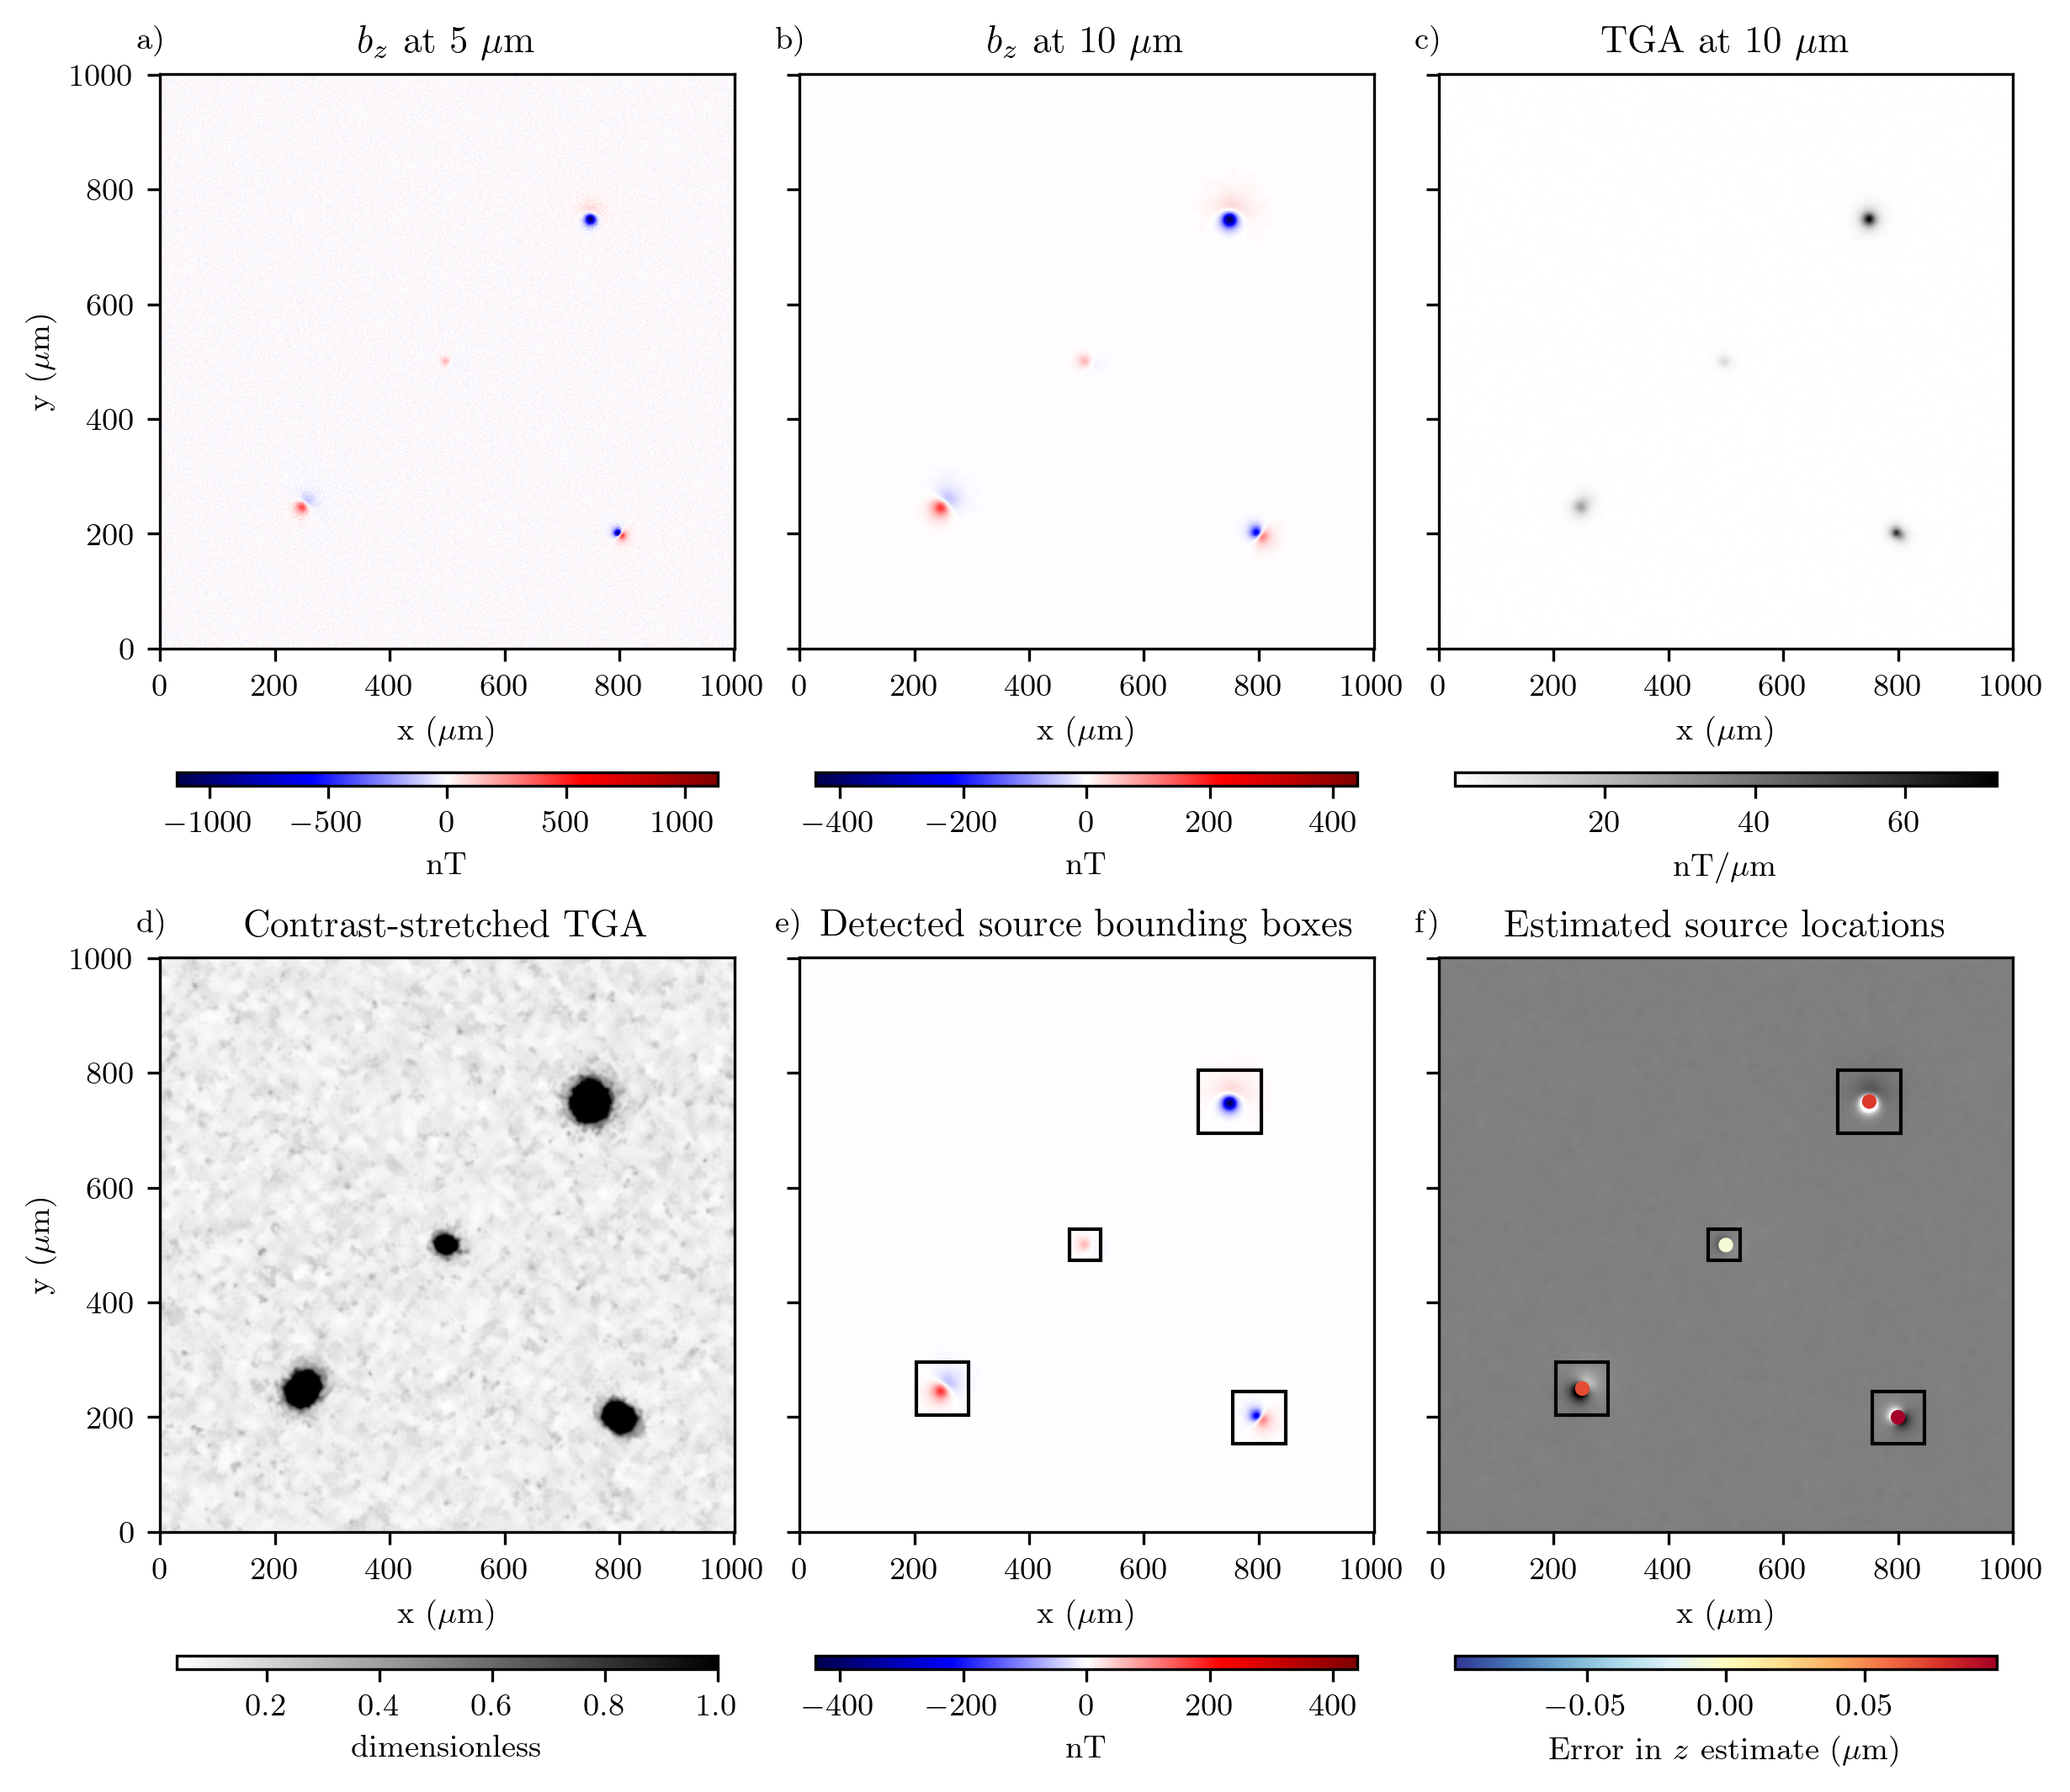
\includegraphics[width=1\linewidth]{figures/simple-synthetic-data.png}
  \caption{
    Simple synthetic data and the various processing steps performed prior to the dipole moment inversion.
    a) The synthetic noise-corrupted $b_z$ observations at
    $z = \qty{5}{\micro\meter}$ due to four dipolar sources with different
    depths and dipole moment vectors
    (see Table~\ref{tab_synthetic_simple_results}).
    b) The upward-continued data to $z = \qty{10}{\micro\meter}$ showing
    attenuated short-wavelength noise.
    c) The total gradient amplitude (TGA) calculated from the
    upward-continued data, which is able to concentrate the signal on top
    of each dipolar source.
    d) The contrast-stretched TGA, highlighting the signal of all four
    sources, including the weak central source.
    e) The detected source bounding boxes (black squares) that correctly
    identify the signal of all four sources.
    f) The estimated source locations (colored circles) from Euler
    deconvolution of the upward-continued data inside each bounding box.
    The color represents the difference between the true and the estimated
    $z$ coordinates.
  }
  \label{fig_synthetic_simple_data}
\end{figure}

Figure~\ref{fig_synthetic_simple_data}a shows the vertical component of the magnetic field $b_z$ over a synthetic rock section containing four dipolar sources.
The map covers a surface of $\qty{1000}{\um} \times \qty{1000}{\um}$, with data points in a regular grid with approximately \qty{1}{\um} spacing ($N = 10^6$ observations) obtained at a sensor-sample distance of \qty{5}{\um}.
The magnetic field data are contaminated with pseudo-random Gaussian noise with zero mean and \qty{20}{\nano\tesla} standard deviation.

We first applied an upward continuation filter (Figure~\ref{fig_synthetic_simple_data}b) to smooth out the high-frequency noise \citep{Blakely1996}.
This is important because noise strongly affects the first derivatives of the field, which are required for the source detection algorithm and the Euler deconvolution.
Then, we calculated the total gradient amplitude (Figure~\ref{fig_synthetic_simple_data}c), which was subjected to contrast stretching to highlight the weaker intensity sources as much as possible (Figure~\ref{fig_synthetic_simple_data}d).
Subsequently, we applied the blob detection algorithm to the contrast-stretched total gradient amplitude to obtain the position of the data windows for each source (Figure~\ref{fig_synthetic_simple_data}e).
Euler deconvolution was then performed for each data window identified by assuming a structural index $\eta = 3$ of a point source, therefore obtaining the Cartesian coordinates (Figure~\ref{fig_synthetic_simple_data}f) of each source. For comparison, Table~\ref{tab_synthetic_simple_results} shows the true and estimated values of the source coordinates.

\begin{table}[tb!]
  \begin{center}
    \small
    
\begin{tabular}{ r c c c l l l } 
  \toprule
  & \multicolumn{3}{c}{Position} & \multicolumn{3}{c}{Dipole moment} \\
  & $x_c$ ($\mu$m) & $y_c$ ($\mu$m) & $z_c$ ($\mu$m) & $I$ (\textdegree) & $D$ (\textdegree) & $m$ (A.m²) \\
  \midrule
  true & 800.00 & 200.00 & -3.50 & 22.00 & 125.00 & 5.000e-15 \\
  estimated & 799.91 & 199.94 & -3.40 & 22.08 ± 0.01 & 125.52 ± 0.02 & 4.921e-15 ± 1.4e-18 \\
  true & 750.00 & 750.00 & -8.50 & 62.00 & 10.00 & 1.500e-14 \\
  estimated & 749.98 & 749.99 & -8.43 & 62.00 ± 0.01 & 9.30 ± 0.02 & 1.486e-14 ± 1.8e-18 \\
  true & 250.00 & 250.00 & -10.00 & -30.00 & -140.00 & 1.000e-14 \\
  estimated & 250.03 & 249.89 & -9.93 & -30.32 ± 0.01 & -139.70 ± 0.02 & 9.966e-15 ± 2.6e-18 \\
  true & 500.00 & 500.00 & -7.75 & -50.00 & -70.00 & 2.000e-15 \\
  estimated & 500.07 & 499.95 & -7.76 & -48.66 ± 0.05 & -70.36 ± 0.09 & 2.000e-15 ± 1.8e-18 \\
  \bottomrule
\end{tabular}

  \end{center}
  \caption{
    True and estimated source positions and dipole moments for the method validation test through a simple synthetic data application.
  }
  \label{tab_synthetic_simple_results}
\end{table}

\begin{figure}[tb!]
  \centering
  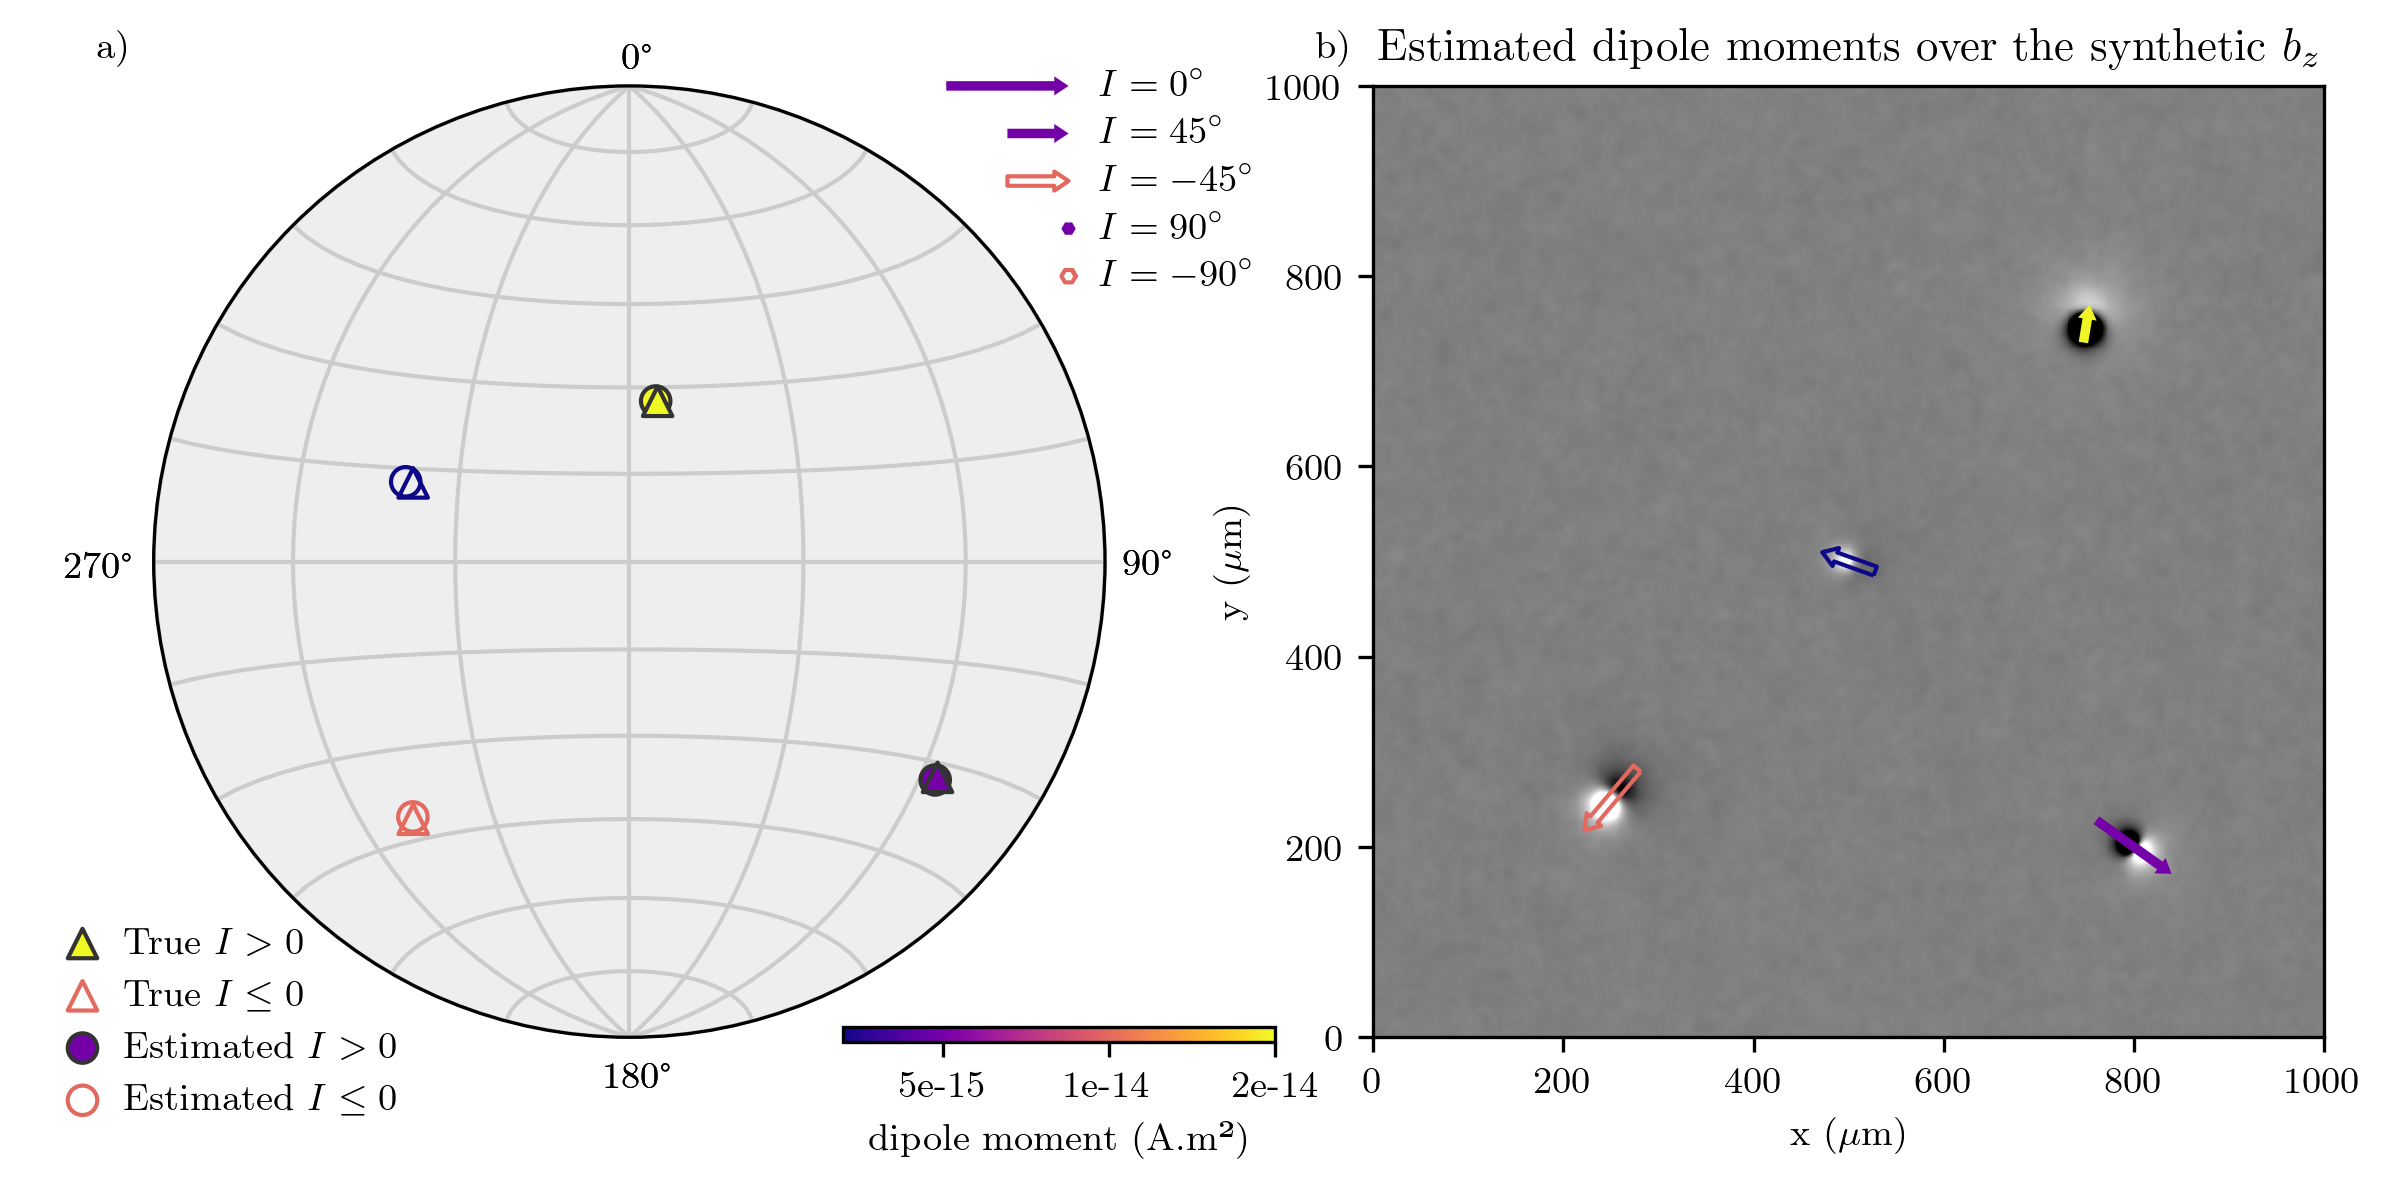
\includegraphics[width=\linewidth]{figures/simple-synthetic-dipole-moment.png}
  \caption{
    Comparison of true and estimated dipole moments for the method validation test through a simple synthetic data application.
    a) Stereonet showing the true (triangles) and estimated (circles) dipole moments.
    The colors are mapped to the dipole moment amplitude.
    b) Grayscale map of the synthetic $b_z$ overlaid by the estimated dipole moment vectors.
    The vector locations were derived from the Euler deconvolution results, their size is inversely proportional to the inclination $I$, their direction represents the declination $D$, and their colors are mapped to the dipole moment amplitude using the same colorscale as the stereonet.
    In both graphs, solid symbols represent positive inclination while hollow symbols represent negative inclination.
  }
  \label{fig_synthetic_simple_results}
\end{figure}

The positions of each source obtained with Euler deconvolution were then used as input for the dipole moment inversion.
The estimated dipole moment vectors are shown in Figure~\ref{fig_synthetic_simple_results}.
Figure~\ref{fig_synthetic_simple_results}a shows the estimated dipole moment, along with the corresponding true values, as a stereonet for better comparison of the true and estimated vector directions.
Figure~\ref{fig_synthetic_simple_results}b shows the estimate dipole moments overlaid on a map of the synthetic $b_z$ to demonstrate the ability of our method to estimate a spatial distribution of dipole moments.
For comparison, Table~\ref{tab_synthetic_simple_results} also shows the true and estimate dipole moments as well as their corresponding standard deviations obtained using Equations~\ref{eq_chi_square}-\ref{eq_variances}.



\subsection{Applicability to non-dipolar sources}

Typically, when conducting magnetic field measurements with a large distance between the sensor and the magnetic anomaly source, higher-order non-dipole magnetization components such as quadrupoles and octupoles can be disregarded because of the strong attenuation with distance of the magnetic fields.
However, in magnetic microscopy, where the sensor is positioned only a few microns from the sample, these higher-order components might be detected.
This phenomenon is observed in paleomagnetic studies on particles with a PSD domain state, where magnetization is non-uniform throughout the grain.
To assess the attenuation of these non-dipolar components and the applicability of our method, we conducted a simulation on particles with more complex magnetization at varying sensor-sample distances.

To simulate particles with non-dipolar magnetization components, we specified a spherical volume with a radius of approximately \qty{1}{\um}.
Within this volume, we added 200 dipolar particles with varying dipole moment directions and amplitudes.
These directions were generated randomly, following a normal distribution centered on the direction $D=\ang{90}$ and $I=\ang{0}$ and with a standard deviation of \ang{10}.
The dipole moment amplitudes were sampled by a normal distribution with mean $\qty{e-14}{\ampere\m\squared}$ and standard deviation $\qty{5e-14}{\ampere\m\squared}$.
We also randomly generated spatial positions around a central position of $x_c=\qty{25}{\um}$, $y_c=\qty{25}{\um}$, and $z_c=\qty{-1}{\um}$ with standard deviation of \qty{0.65}{\um}.
The bulk magnetization of the non-dipolar particle is the vector sum of the dipole moments of each dipole.
The centroid of the particle is defined by the average of the $x_c$, $y_c$, and $z_c$ positions of each dipole.
The synthetic vertical magnetic field $b_z$ of the non-dipolar source was calculated on regular grids with \qty{0.5}{\um} spacing.
Each grid was located at a different sensor-sample distance $z$, varying between \qty{1}{\um} and \qty{10}{\um} in \qty{0.5}{\um} increments.
The synthetic data were corrupted by pseudo-random Gaussian noise of mean \qty{0}{\nano\tesla} and a standard deviation of \qty{20}{\nano\tesla}.
For each data grid generated, we performed Euler deconvolution to estimate the source position and subsequently inverted the data for the dipole moment.
At each step, we recorded the inversion $R^2$ value and the differences between the estimated position and dipole moment and the true centroid and bulk magnetization of the particle.

Figure~\ref{non-dipolarity-synthetic-data} shows the synthetic $b_z$ of an example non-dipolar particle at variable source-sample distances.
When the particle is close to the sensor (\qtyrange{1}{3}{\um}), the observed field is strongly non-dipolar (Figure~\ref{non-dipolarity-synthetic-data}a-b) and the dipole moment inversion produces low $R^2$ values.
As the distance increases, the magnetic field is attenuated, particularly the non-dipolar components which decay more rapidly than the dipolar component.
This results in an increase in $R^2$ (Figure~\ref{non-dipolarity-synthetic-data}c-d).
At distances above \qty{5}{\um}, there is practically only the contribution of the dipolar component, causing $R^2$ to approach its maximum value of 1 (Figure~\ref{non-dipolarity-synthetic-data}e-f).

\begin{figure}[tb!]
  \centering
  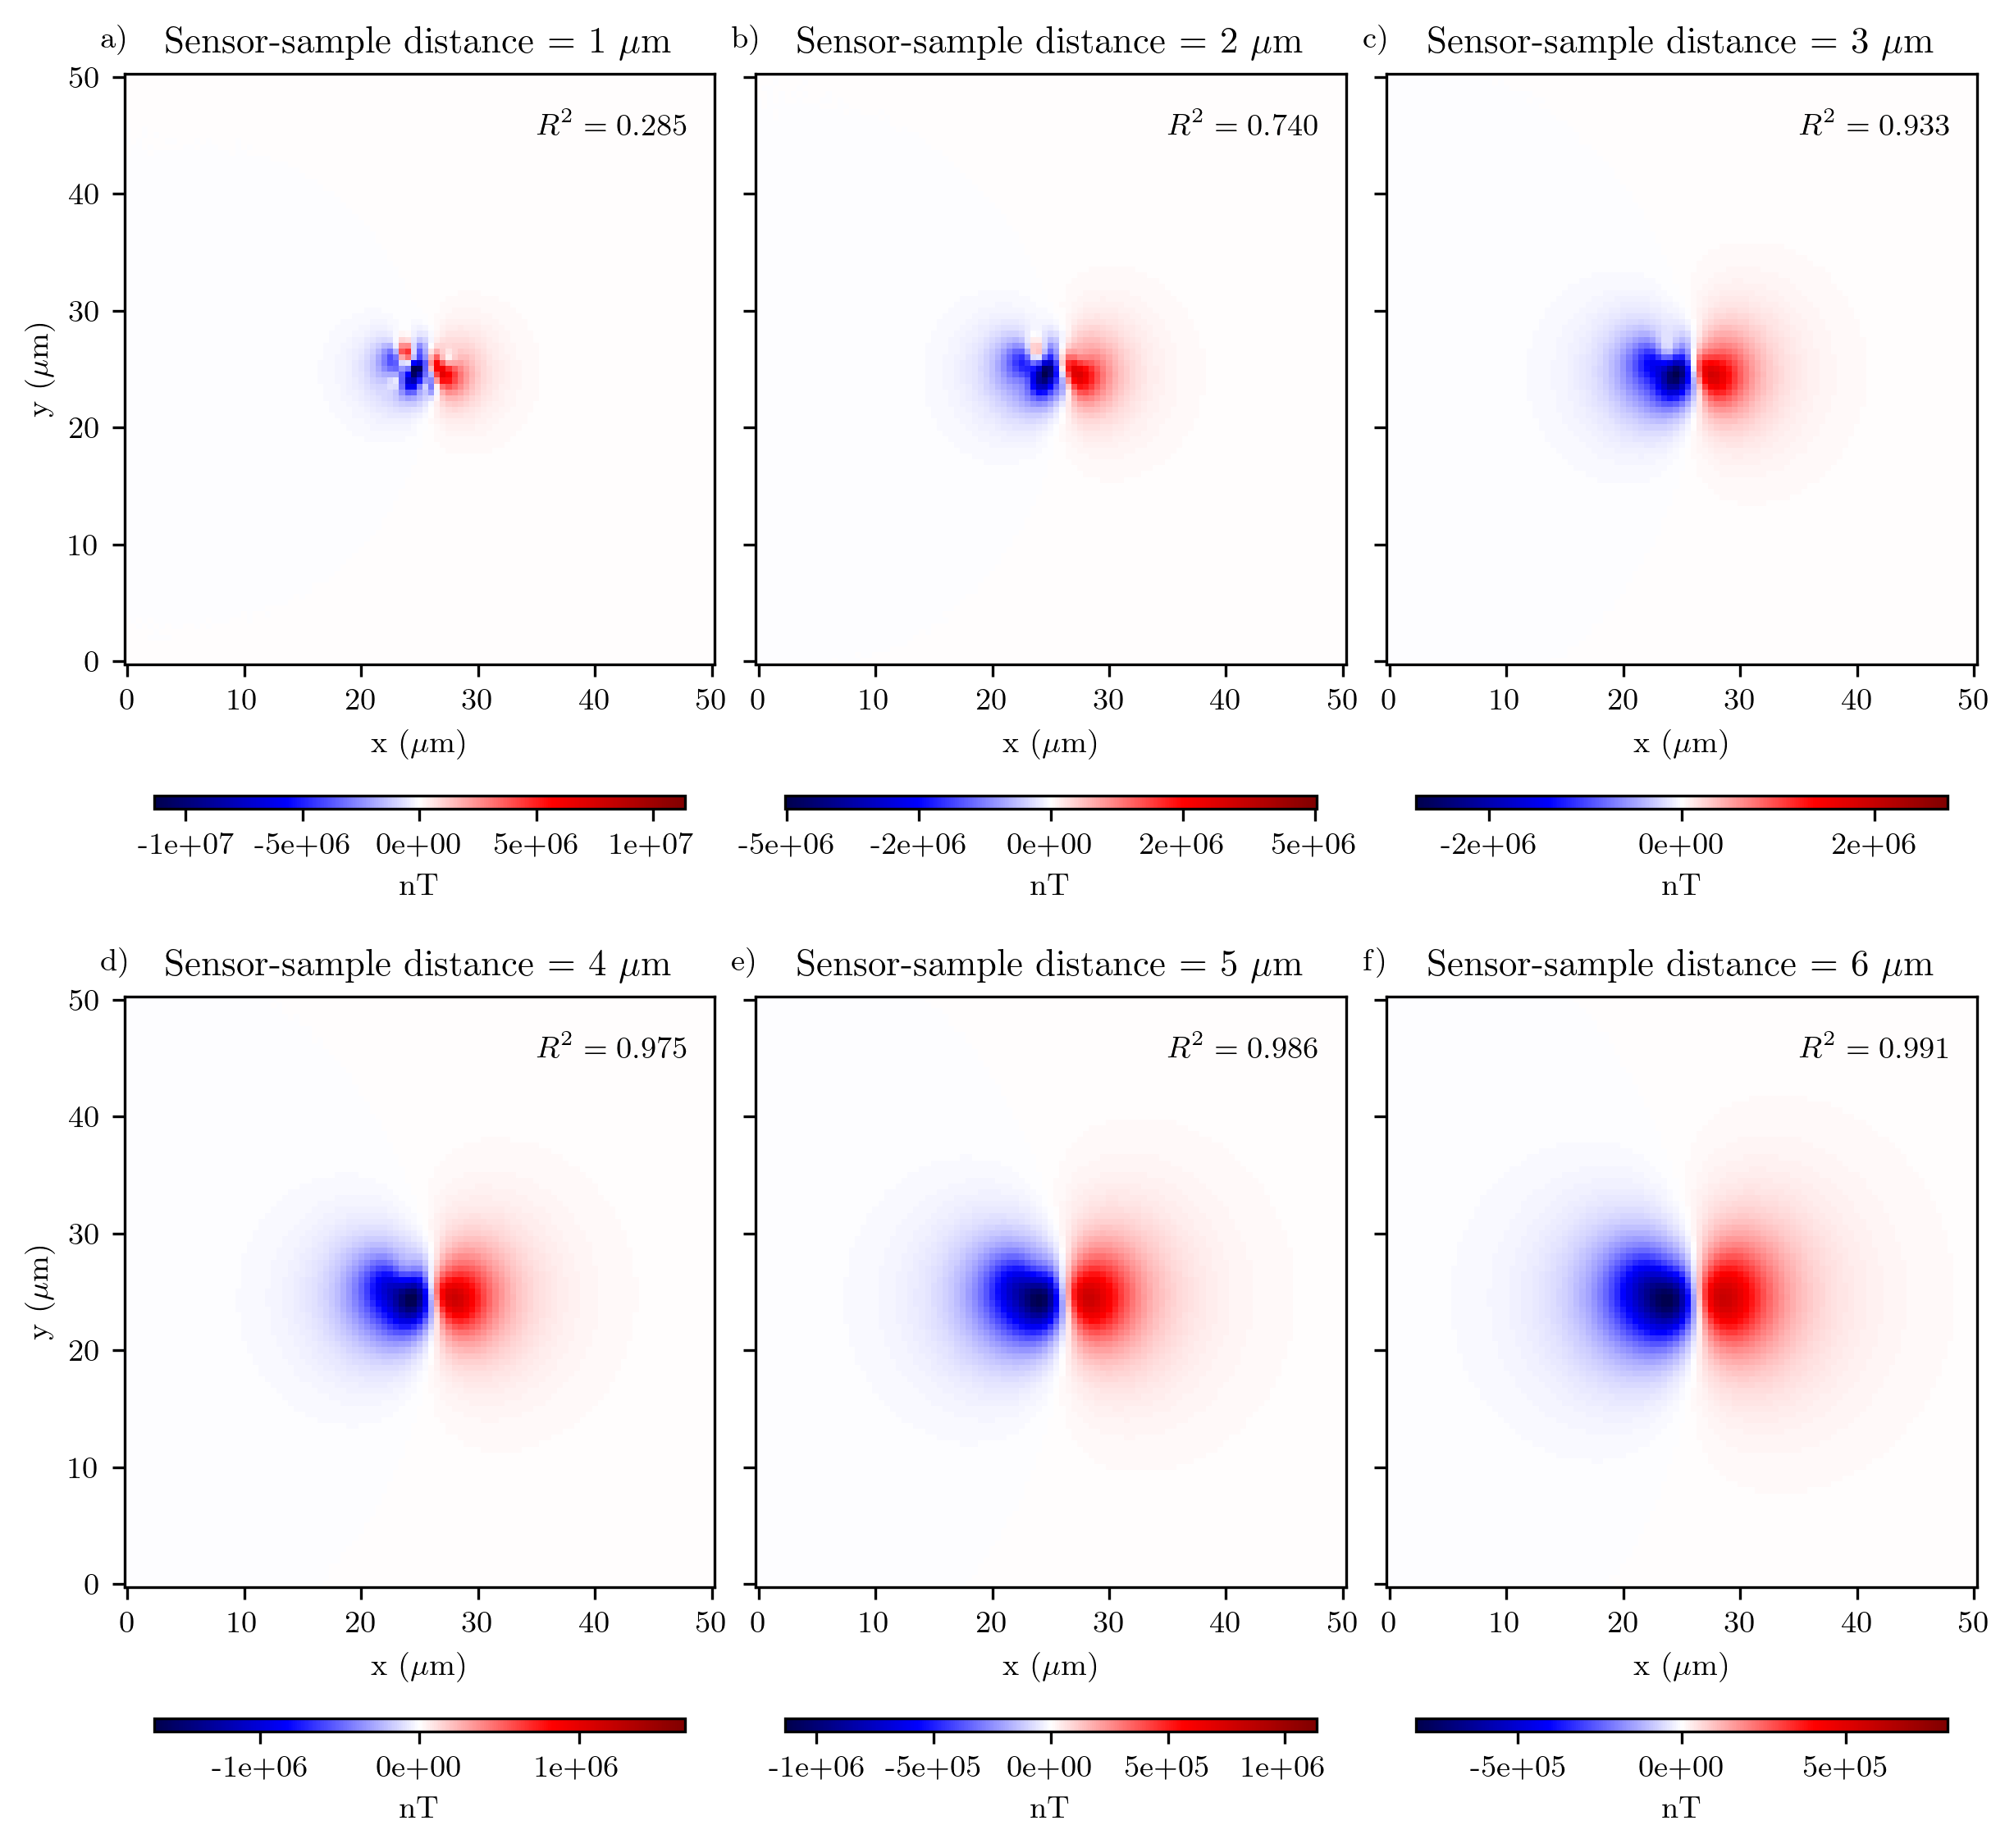
\includegraphics[width=1\linewidth]{figures/non-dipolarity-synthetic.png}
  \caption{Caption: Simulated magnetic microscopy data for a spherical source with both dipolar and non-dipolar magnetic components. The distance from the sensor varies from 1 µm to 6 µm (a-f).}
  \label{non-dipolarity-synthetic-data}
\end{figure}

We replicated the particle generation procedure 100 times with variations in the randomness of magnetization and point particle positions. Subsequently, the Cartesian position of the spherical particle was estimated using ED, and the magnetization parameters were determined by inverting the magnetic field data. The effectiveness of position recovery was measured by comparing the particle's centroid with the solution of the Euler equation for $x_c$, $y_c$, and $z_c$ (Figure~\ref{non-dipolarity-synthetic-data-positioning}a, b, and c, respectively). As shown in Figure~\ref{non-dipolarity-synthetic-data-positioning}, ED estimates the positions of particles with more complex magnetization well, especially for sensor-source distances greater than 5 µm, where the median of the distributions is centered at zero. However, when the sensor-source distance is small enough to emphasize the contribution from higher-order components, a lower degree of dipolarity is observed as expressed by lower values of $R^2$ (Figure~\ref{non-dipolarity-synthetic-data-inversion}a). Consequently, in these cases, there are higher errors in the estimation of the direction of magnetization (Figure~\ref{non-dipolarity-synthetic-data-inversion}b) and in the magnetic moment's intensity (Figure~\ref{non-dipolarity-synthetic-data-inversion}c), which were expected since the inversion considers only the dipolar component. However, dipolarity significantly increases as the sensor to sample distance increases, while errors in direction and magnetic moment decrease significantly (Figure~\ref{non-dipolarity-synthetic-data-inversion}).

\begin{figure}[tb!]
  \centering
  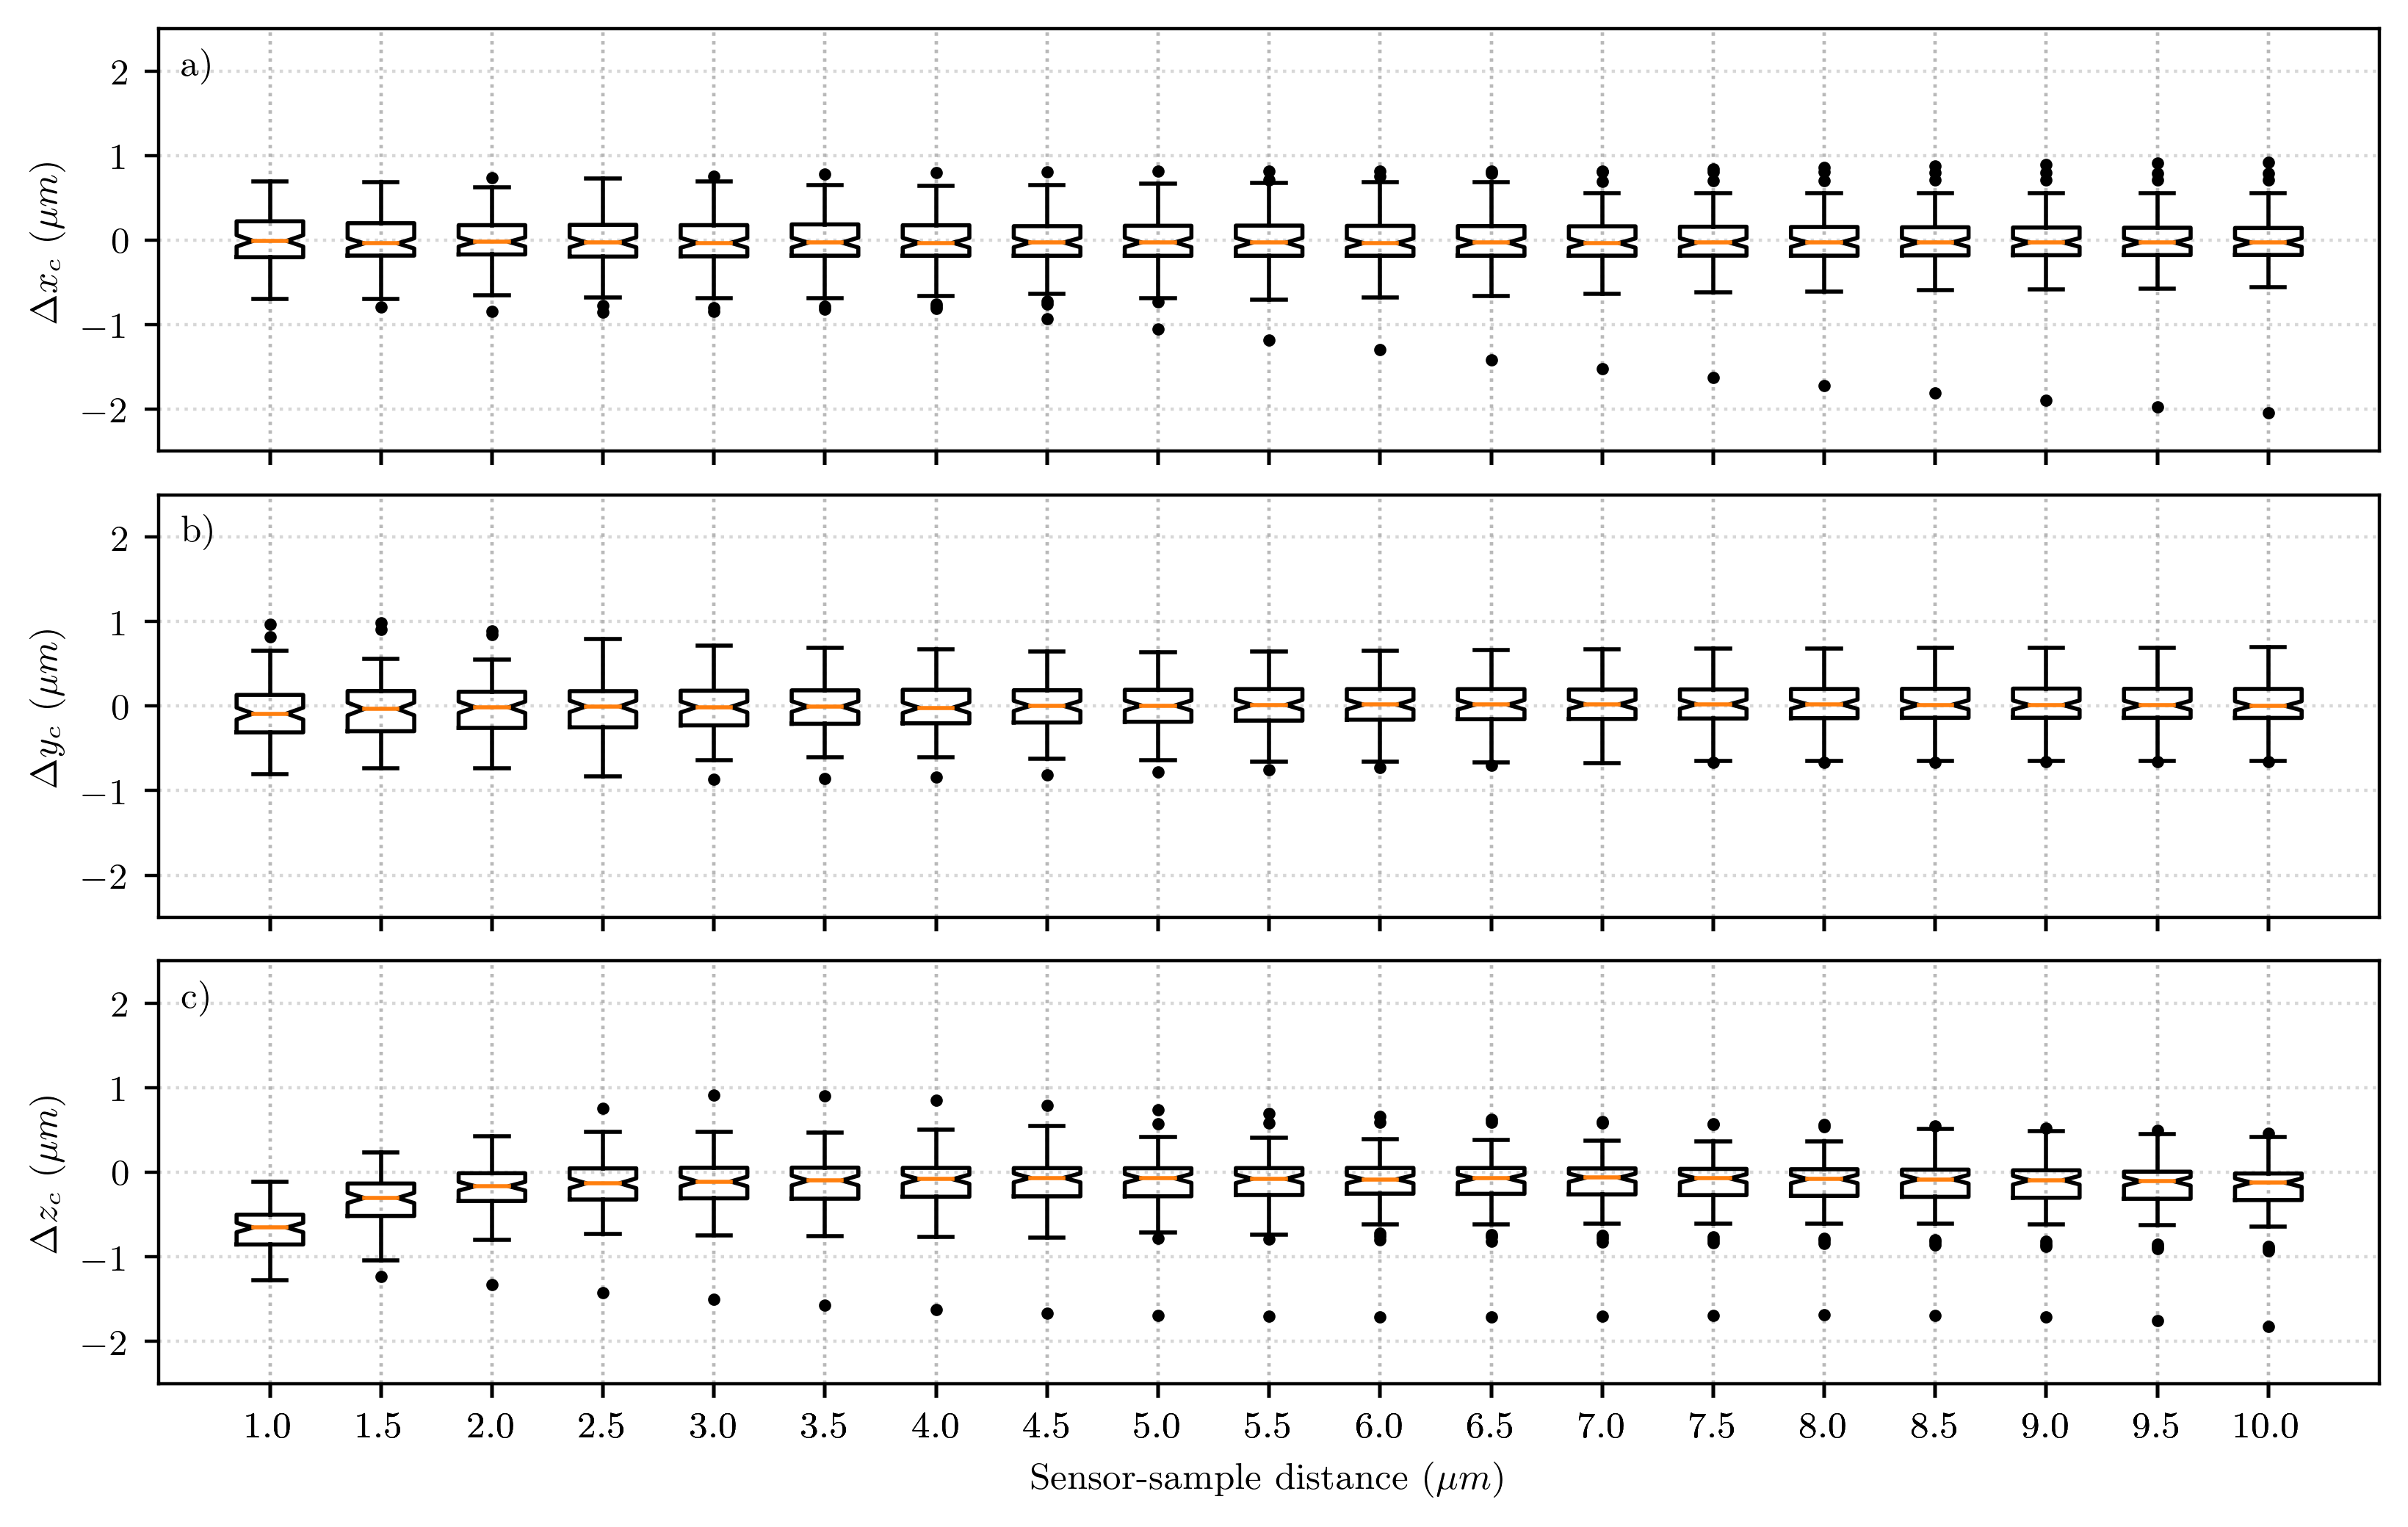
\includegraphics[width=1\linewidth]{figures/non-dipolarity-synthetic-positioning.png}
  \caption{The simulation was randomly replicated (N=100) to test the effectiveness of the Euler deconvolution in estimating the position of the modeled particles. The difference between the true position (centroid) and the estimated position was calculated for each replicate and plotted as a boxplot. The boxplot shows the distribution of differences in the (a) $x_c$, (b) $y_c$, and (c) $z_c$.}
  \label{non-dipolarity-synthetic-data-positioning}
\end{figure}

\begin{figure}[tb!]
  \centering
  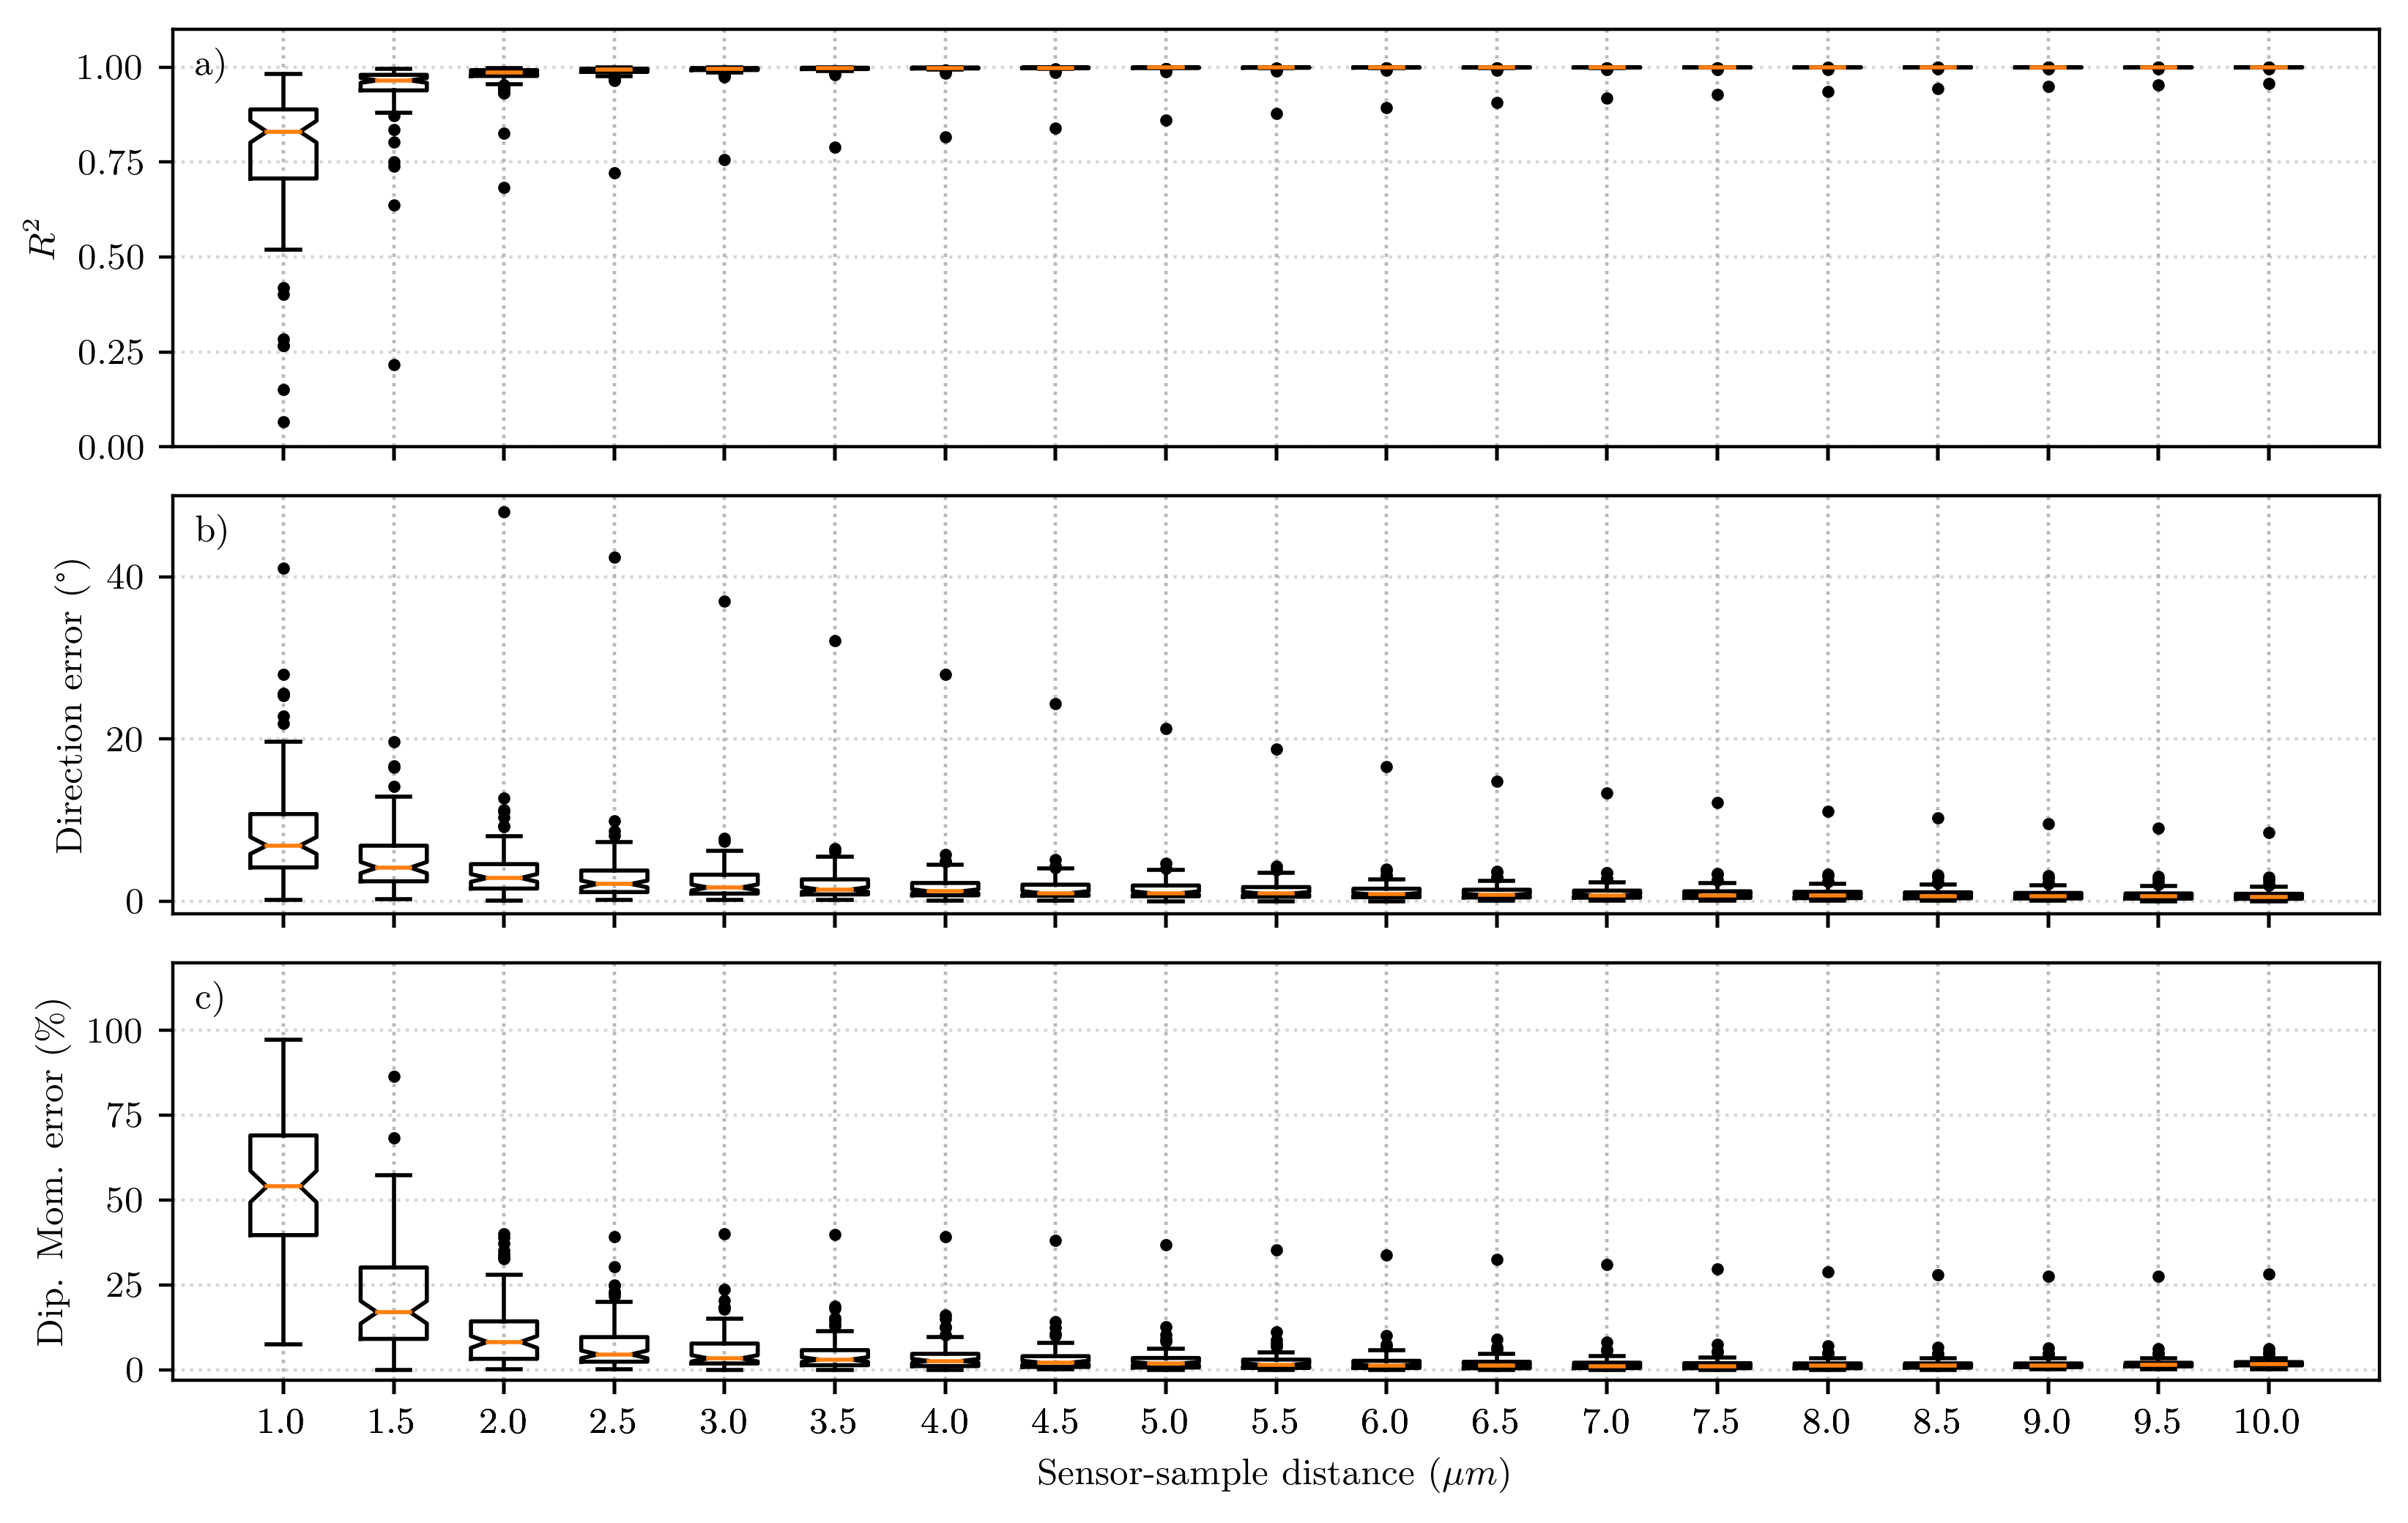
\includegraphics[width=1\linewidth]{figures/non-dipolarity-synthetic-inversion.png}
  \caption{The simulation was randomly replicated (N=100) to assess the accuracy of the algorithm in recovering the magnetic direction and moment of the modeled particles. The goodness of fit was measured by the R-squared value (a), while the angular error (b) and intensity error (c) between the real and modeled magnetic vector were plotted in degrees and percentages ($|100 \left( m_{true} - m_{estimated}\right) ~/~ m_{true}|$), respectively.}
  \label{non-dipolarity-synthetic-data-inversion}
\end{figure}



\subsection{Applicability to real-world scenarios}\label{complex-synthetic-section}

This test represents a more complex scenario by simulating 103 sources randomly distributed in the imaged area of a synthetic thin section of $\qty{2000}{\um} \times \qty{2000}{\um}$.
The synthetic $b_z$ data were generated on a regular grid with $\qty{2}{\um}$ spacing and $\qty{5}{\um}$ sensor-sample distance.
We contaminated the data with high-frequency normally-distributed pseudo-random noise with zero mean and $\qty{50}{\nano\tesla}$ standard deviation, as well as with low-frequency noise in the form of additional deep sources beyond the modeling domain.

For greater fidelity to real samples, the magnetic sources are modeled as dipoles with different depths and magnetic moment intensities.
The depths vary randomly between 1 and $\qty{20}{\um}$, while the dipole moment intensities range randomly from $10^{-12}$ to $10^{-14}{Am^2}$.
The NRM found in real ferromagnetic particles varies individually but averages out to the inducing field direction.
To simulate this behavior in our synthetic data, we sample the source dipole moment directions from two pseudo-random Gaussian distributions.
The first group of sources ($M = 70$) are sampled from a distribution  with mean of $D = \ang{0}$ and $I = \ang{0}$ and standard deviation of $\ang{10}$.
The second group of sources ($M = 30$) are sampled from a distribution with mean of $D = \ang{180}$ and $I = \ang{0}$, also with standard deviation of $\ang{10}$. We also manually added 3 sources with higher dipole moments ($5$x$10^{-11}$) to further simulate the complexity observed in real data measurements. The noise-corrupted synthetic $b_z$ data are shown in Figure~\ref{complex-synthetic-data}a.

\begin{figure}[tb!]
  \centering
  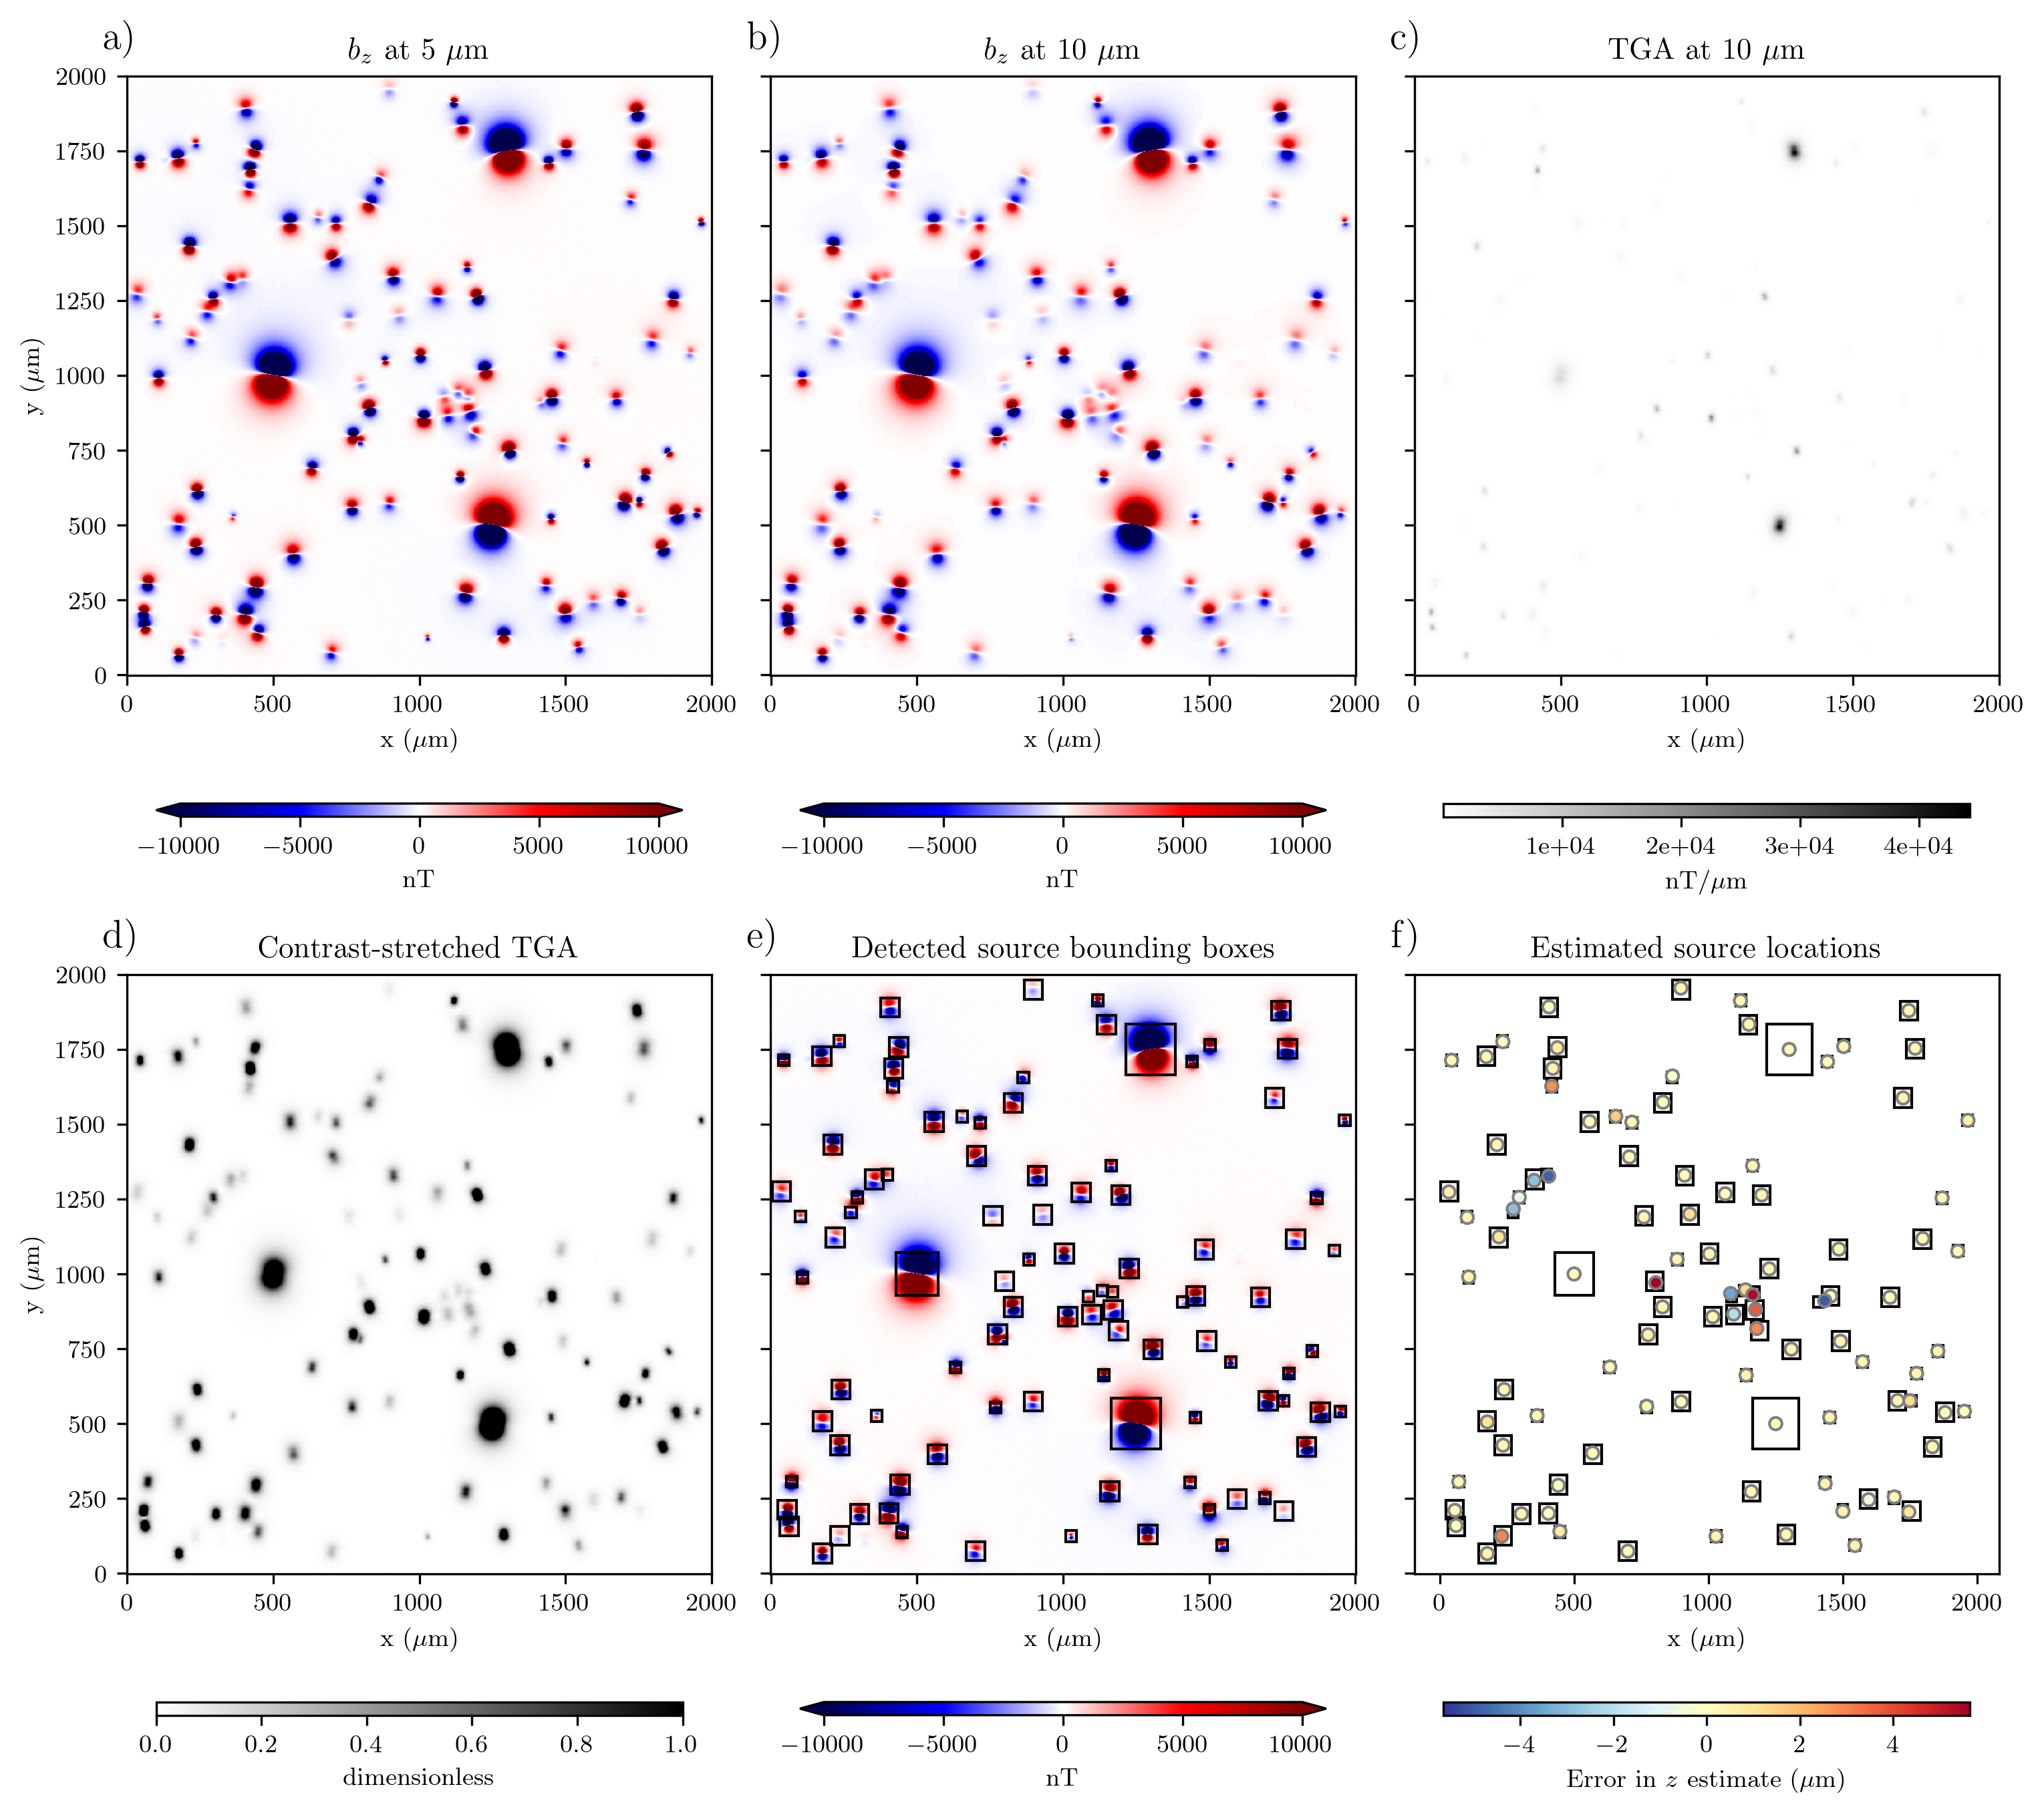
\includegraphics[width=1\linewidth]{figures/complex-synthetic-data.png}
  \caption{
    Complex synthetic data and the various processing steps performed prior to the dipole moment inversion.
    a) The synthetic high and low-frequency noise-corrupted $b_z$ observations at
    $z = \qty{5}{\micro\meter}$ due to two clusters of stable directions simulated.
    b) Anomaly map after the upward-continued data to $z = \qty{10}{\micro\meter}$ to attenuated long and short-wavelength noise.
    c) The total gradient amplitude (TGA) calculated from the
    upward-continued data, which is able to concentrate the signal on top
    of each dipolar source.
    d) The contrast-stretched TGA, highlighting the signal of all sources, especially the weaker ones.
    e) The detected source bounding boxes (black squares) that correctly
    encapsulate the signal of the sources.
    f) The estimated source locations (colored circles) from Euler
    Deconvolution of the upward-continued data inside each bounding box.
    The color represents the difference between the true and estimated
    $z$ coordinates.
  }
  \label{complex-synthetic-data}
\end{figure}

We then followed the same processing steps as for the simple synthetic: upward continuation (Figure~\ref{complex-synthetic-data}b),
TGA calculation (Figure~\ref{complex-synthetic-data}c), contrast stretching (Figure~\ref{complex-synthetic-data}d), blob detection (Figure~\ref{complex-synthetic-data}e), and Euler Deconvolution (Figure~\ref{complex-synthetic-data}e).
A total of 99 sources out of the original 103 were successfully detected by our workflow.

\begin{figure}[tb!]
\centering
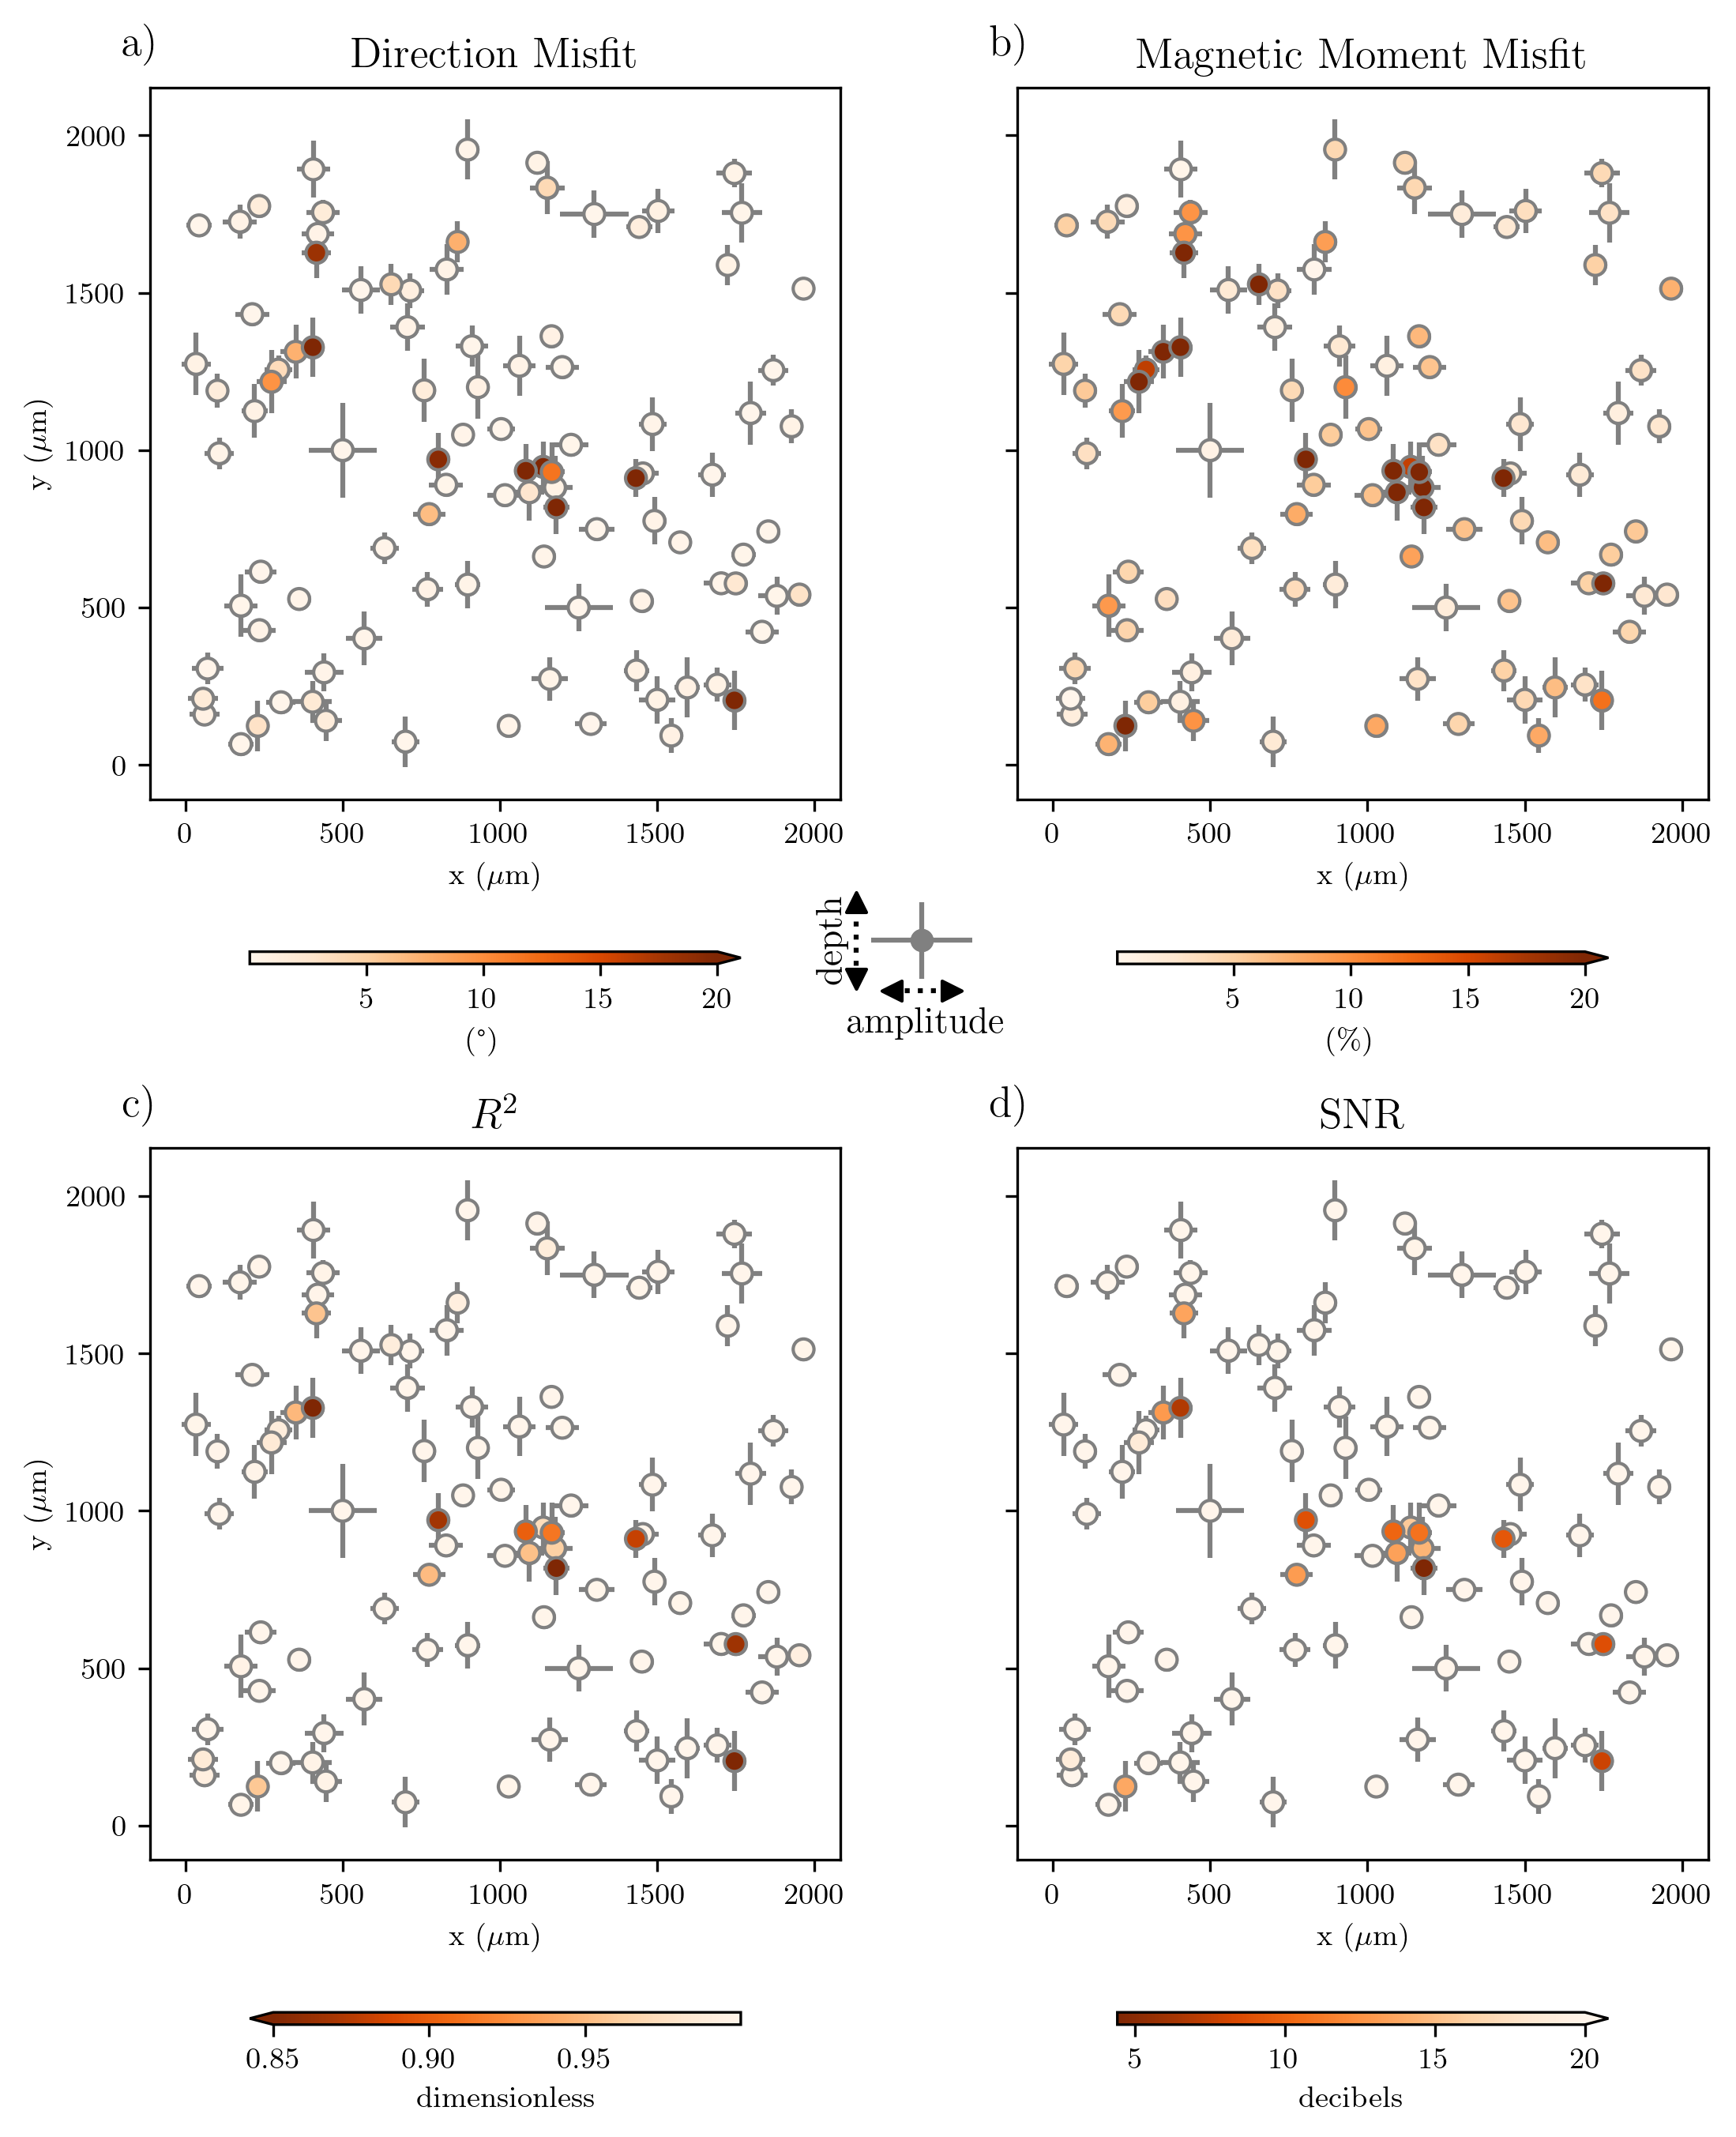
\includegraphics[width=0.75\linewidth]{figures/complex-synthetic-comparison.png}
\caption{
The validation of the result obtained with the inversion was calculated for each individual particle based on the error between the real parameters modeled and their respective recovered values, being (a) the direction and (b) intensity of the magnetic moment, in addition to the $R^2$ score (c) obtained by comparing the forward model and the actual data. The depth and radius of the magnetic sources are also important factors that influence the final result, therefore, these data are given in the form of cross plots, with the vertical bar represented by the depth (1 - 20 $\mu m$) and the horizontal bar by the dipole moment amplitude ($10^{-12}$ to $10^{-14}$ $Am^2$).
}
\label{complex-synthetic-comparison}
\end{figure}

The spatial resolution of the inversion results is one of the key advantages of magnetic microscopy over the classic techniques of paleomagnetism.
Therefore, we present the inversion results spatially so that we can evaluate any patterns in their distribution.
Figure~\ref{complex-synthetic-comparison} shows the spatial locations of the 99 sources that were identified and the differences between the estimated dipole moments and the true values.
The depth and dipole moment amplitude of each source are represented by horizontal and vertical bars, respectively.
These two variables are useful proxies for the strength and spatial extent of the signal of each source,
which can tell us about the limitations in strengths and sizes of the source signal that the technique is able to correctly invert.
Figure~\ref{complex-synthetic-comparison}a shows the absolute value of the angular difference between the true and the estimated dipole moment vectors.
Figure~\ref{complex-synthetic-comparison}b shows the percentage difference between the true and estimated dipole moment magnitudes ($|100 \left( m_{true} - m_{estimated}\right) ~/~ m_{true}|$).
Figure~\ref{complex-synthetic-comparison}c shows the $R^2$ coefficient (Equation~\ref{eq_r2}), which is equivalent to the non-dipolarity parameter of \citet{Fu2020} and represents how well the dipolar model is able to explain the observed data of each source.
Figure~\ref{complex-synthetic-comparison}d shows the SNR (Equation~\ref{eq_snr}), which expresses the power of the observed data over that of the inversion residuals.
High SNR values correspond to small inversion residuals which indicate that a dipolar model was able to explain the observed data.
Consequently, the variation of SNR values is similar to that of the $R^2$ coefficient.
Figure~\ref{complex-synthetic-comparison} shows that large errors in the estimated dipole moment direction are associated with low values of $R^2$ and SNR.
Conversely, the correlation between errors in dipole moment magnititude and $R^2$ and SNR is less pronounced, with some poor magnitude estimates being associated with $R^2$ and SNR indicating a good fit of the dipolar model.
It is also noticeable that the majority of cases where the dipole moment direction error is large are associated with deep and low-amplitude sources that are close to shallower or higher-amplitude sources.
These results indicated that $R^2$ and SNR can be used as selection criteria to discard sources with likely high errors in the estimated dipole moment.

\begin{figure}[tb!]
\centering
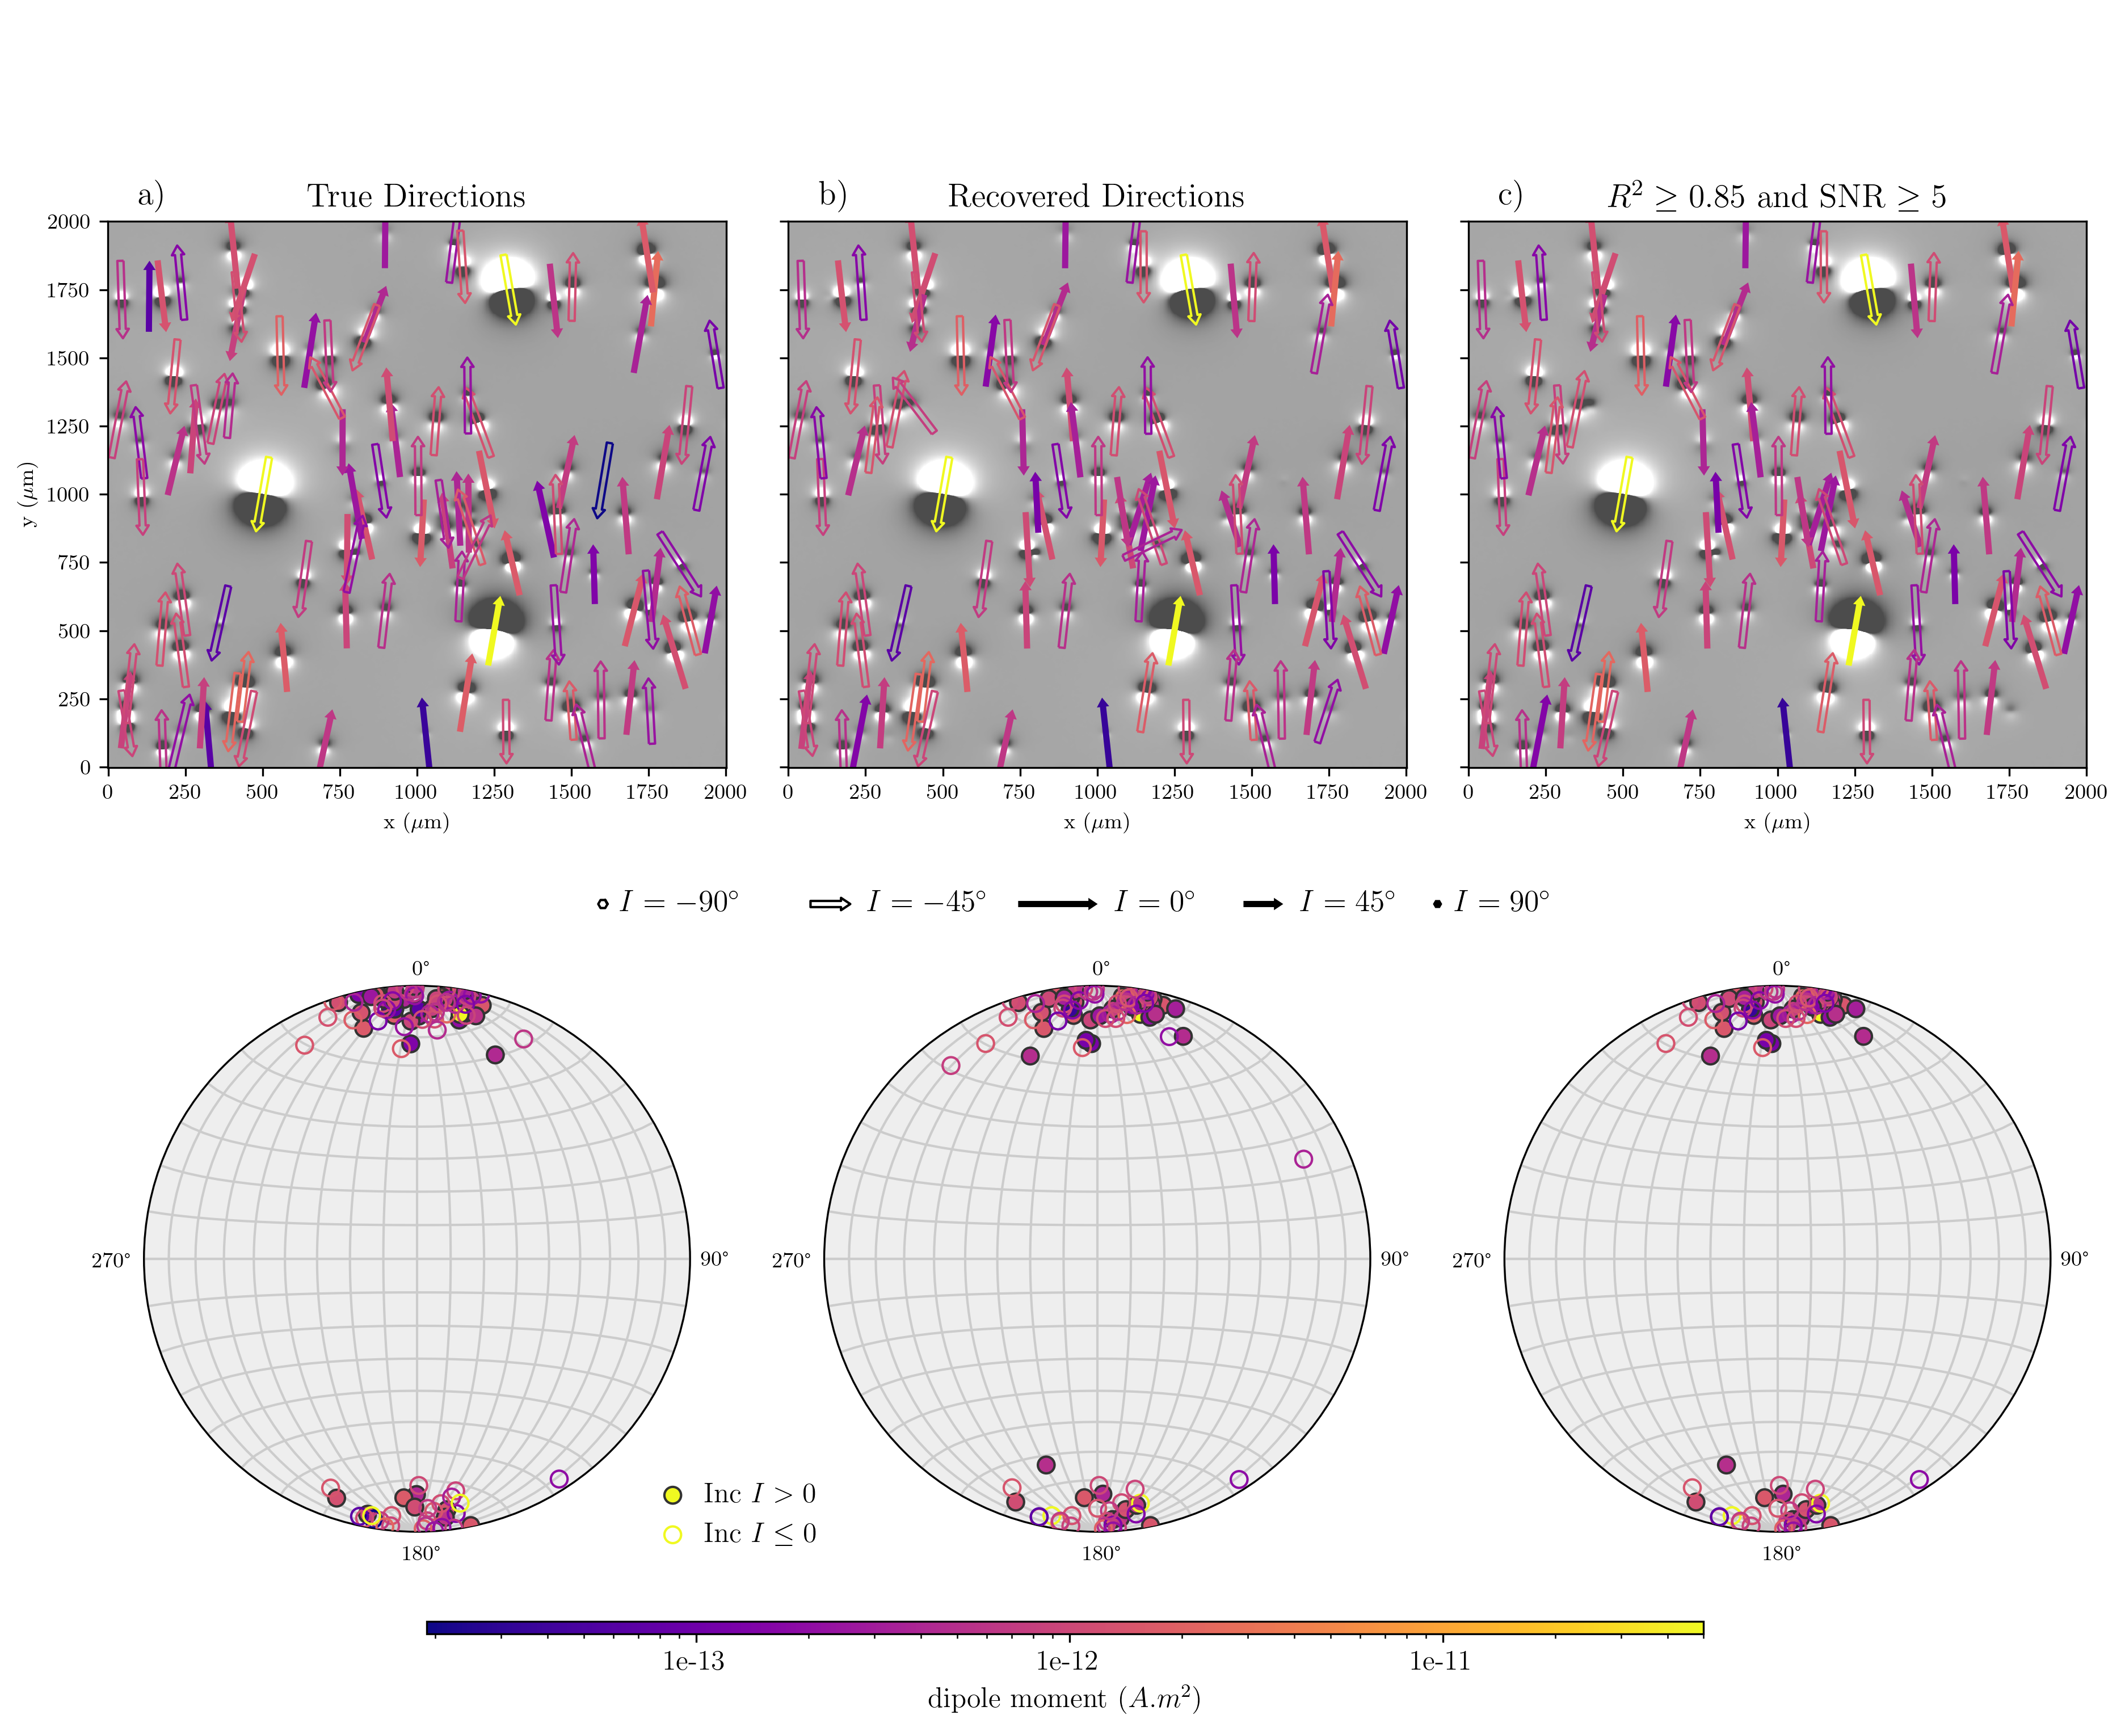
\includegraphics[width=1\linewidth]{figures/complex-synthetic-stereograms.png}
\caption{ Comparison of true and estimated dipole magnetic moments and directions for the complex synthetic sample.
a) Simulation of a thin section of rock with 103 particles uniformly magnetized (dipolar sources) by two different induced fields. The average directions of the induced fields are $D=\ang{0}$ / $I=\ang{0}$ and $D=\ang{180}$ / $I=\ang{0}$, yielding two stable directions. b) All estimated vector directions of the identified sources ($M=99$). c) The Filtering criteria used to select the magnetic directions of the sources with the best fitting ($M=96$), determined by the coefficient of determination ($R^2 \geq 0.85$) and signal-to-noise ratio ($\text{SNR} \geq 5$).
}
\label{complex-synthetic-stereograms}
\end{figure}

Figure~\ref{complex-synthetic-stereograms} shows stereograms with the directions generated by the modeled (Figure~\ref{complex-synthetic-stereograms}a) and the estimated vectors (Figure~\ref{complex-synthetic-stereograms}b) for each source. The distribution of the estimated directions is coincident with the true directions aside from a few sources, the same ones with the higher values of direction misfit (Figure~\ref{complex-synthetic-comparison}a) which is probably associated with the mutual interference of sources close to each other or within the same window. When filtered to include only data with R\textsuperscript{2} \textgreater 0.85 and SNR \textgreater 5 the obtained direction distribution is closer to the true distribution (Figure~\ref{complex-synthetic-stereograms}c).


%%%%%%%%%%%%%%%%%%%%%%%%%%%%%%%%%%%%%%%%%%%%%%%%%%%%%%%%%%%%%%%%%%%%%%%%%%%%%%%
\section{Application to real data}

To test whether the proposed method would be able to determine the
magnetization directions and the magnetic moment of particles in natural
samples, we selected a previously studied carbonate stalagmite sample from the
Wintimdouine cave in the Agadir region (Morocco) \citep{Ait2019Hydro}. This
speleothem contains both magnetite and hematite as the main carriers of
magnetic remanence, as attested by thermomagnetic curves with temperature
decays at {\textasciitilde}580 °C and {\textasciitilde}680 °C, and bimodal
curves of isothermal remanent magnetization (IRM) acquisition \citep{carmo2019speleothem}.

In order to provide two distinct directions associated with the different
magnetic mineral types in this sample, we applied two IRM pulse fields of 2.7 T
and 0.3 T, respectively toward the +Y and -Y directions. In this way, the high
coercivity grains (hematite) would point towards +Y and the low coercivity ones
(magnetite) would align in the -Y direction.

After remanence acquisition, we performed a magnetic map with the Quantum
Diamond Microscope (QDM) at Harvard University over a sample section of
approximately $\qty{1410}{\um} \times \qty{2256}{\um}$ (Figure~\ref{real-data}a) with a grid
spacing of \qty{2.35}{\um} and a sensor-sample distance of approximately \qty{5}{\um}, totaling
576,000 data points. The QDM is housed in a shielded room, in
order to avoid the influence of the Earth's magnetic field while the data were taken in projected magnetic microscopy (PMM) mode and converted to the vertical component of magnetic field ($b_z$) using a spectral approach \citep{Lima2009, Fu2020,
Glenn2017}. We applied a bias field of \qty{0.9}{\milli\tesla} during the measurement, which was periodically reversed to result in an effective background field of $< \qty{1}{\micro\tesla}$.  After applying the magnetic anomaly detection algorithm (Figure~\ref{real-data}b-e), it was
possible to determine the windows for 75 potential sources, as shown in Figure~\ref{real-data}e.

\begin{figure}[tb!]
\centering
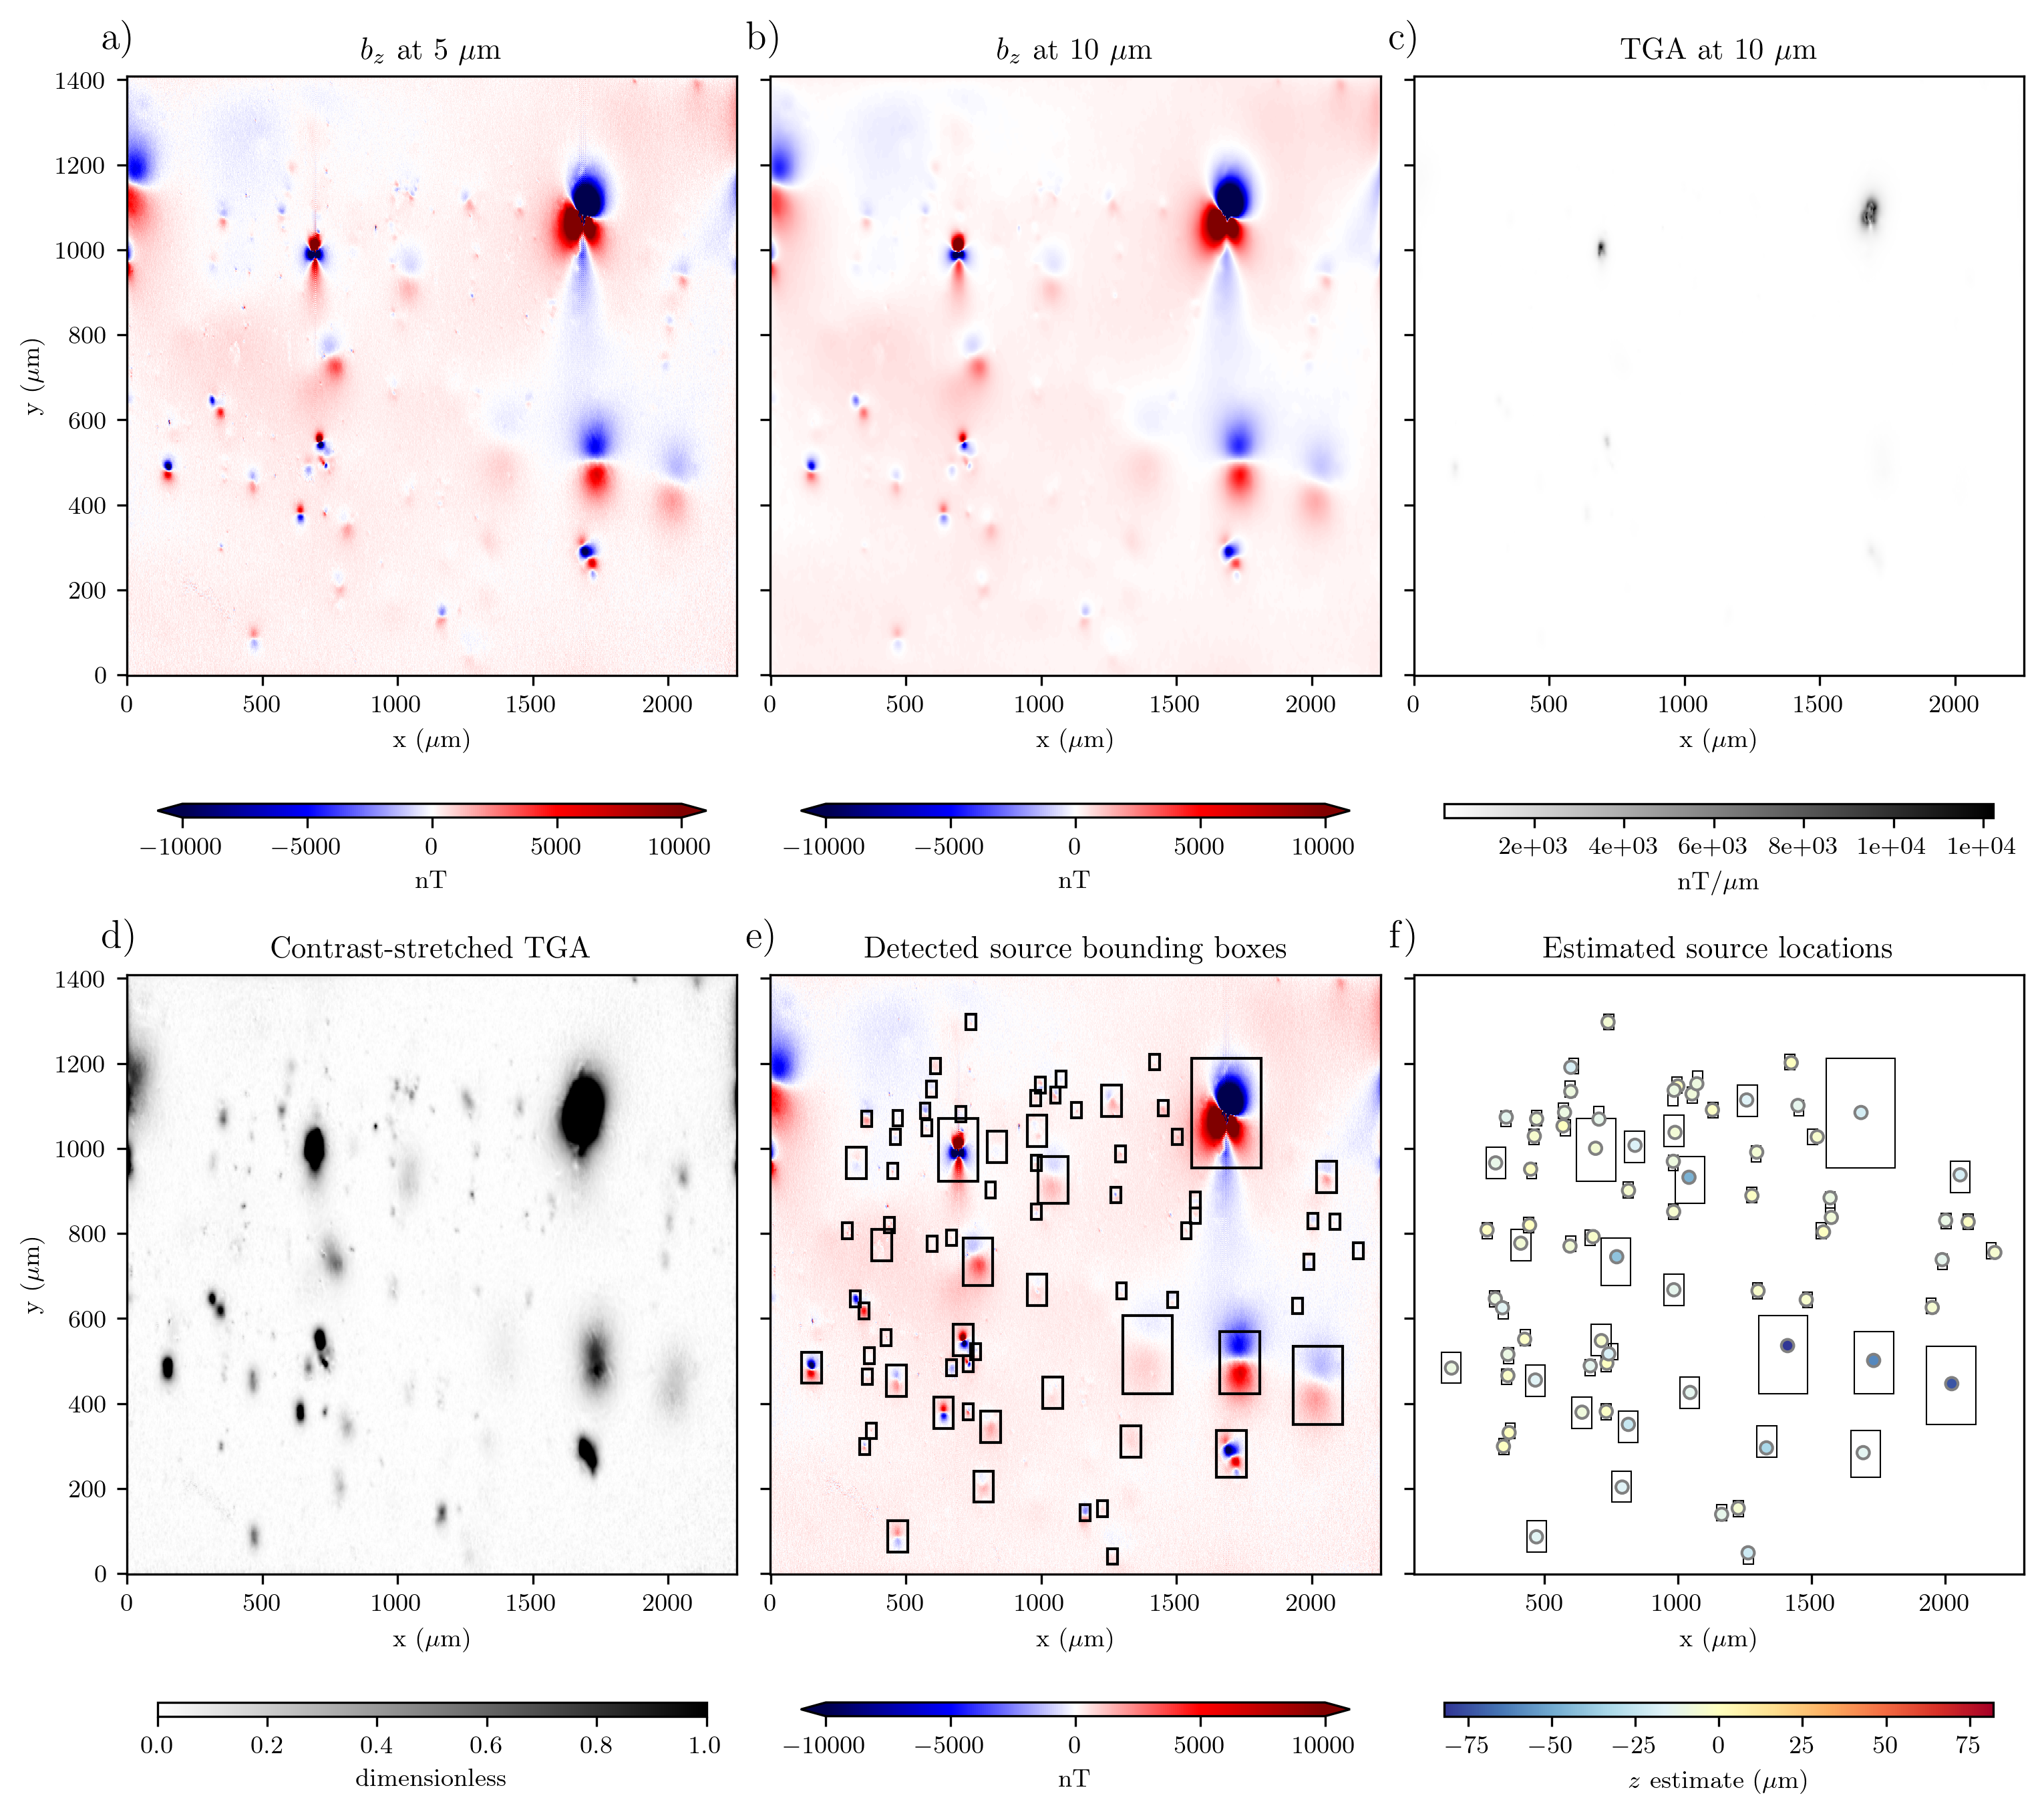
\includegraphics[width=1\linewidth]{figures/real-data.png}
\caption{Real data and the various processing steps performed prior to the dipole moment inversion.
    a) The real sample vertical component magnetic data $b_z$ observations at
    $z = \qty{5}{\um}$.
    b) Anomaly map after the upward-continued data to $z = \qty{10}{\um}$ to attenuated long and short-wavelength noise.
    c) The total gradient amplitude (TGA) calculated from the
    upward-continued data.
    d) The contrast-stretched TGA.
    e) The detected source bounding boxes (black squares) that correctly
    encapsulate the main signal of the sources.
    f) The estimated source locations (colored circles) from Euler
    Deconvolution of the upward-continued data inside each bounding box.
    The color represents the estimated $z$ coordinates.
  }
\label{real-data}
\end{figure}

After applying the ED algorithm, we performed the inversion of the magnetic moment for each of the 75 windows selected previously. In order to reduce considerably the computation time, the inversions were done within each data window, instead of solving all sources parameters at the same time. We obtained the magnetic moment and the direction for all 75 magnetic grains (Figure~\ref{real-data-stereograms}a). Then, we calculated the residuals of the inversions in each window and subsequently the coefficient of determination $R^2$ and signal-to-noise ratio (SNR), which were parameters used as filters for the best directions obtained. We considered a good fit to be achieved when $R^2$ was greater or equal to 0.85 and SNR was greater than 5. An $R^2$ value of 0.85 indicates that \qty{85}{\percent} of the measured magnetic data is explained by the predicted dipole model, which is equivalent to the dipolarity test approach \citep{Fu2020}. On the other hand, an SNR of 5 means that the dipolar signal is 5 times greater than the residual noise. By using these criteria, we ensured that the fit was sufficiently accurate and the dipole model provided a reliable approximation of the original magnetic data. About 46 identified sources passed these criteria. This filtering technique removed the poorly fit predicted models as well as the ones too corrupted with noise, showing more clearly the expected directional clusters of hematite and magnetite crystals (Figure~\ref{real-data-stereograms}b). Notably, it is confirmed that the sample has both magnetic minerals, but by the expected directions we can also stipulate that the magnetite grains outnumber the hematite ones.

\begin{figure}[tb!]
\centering
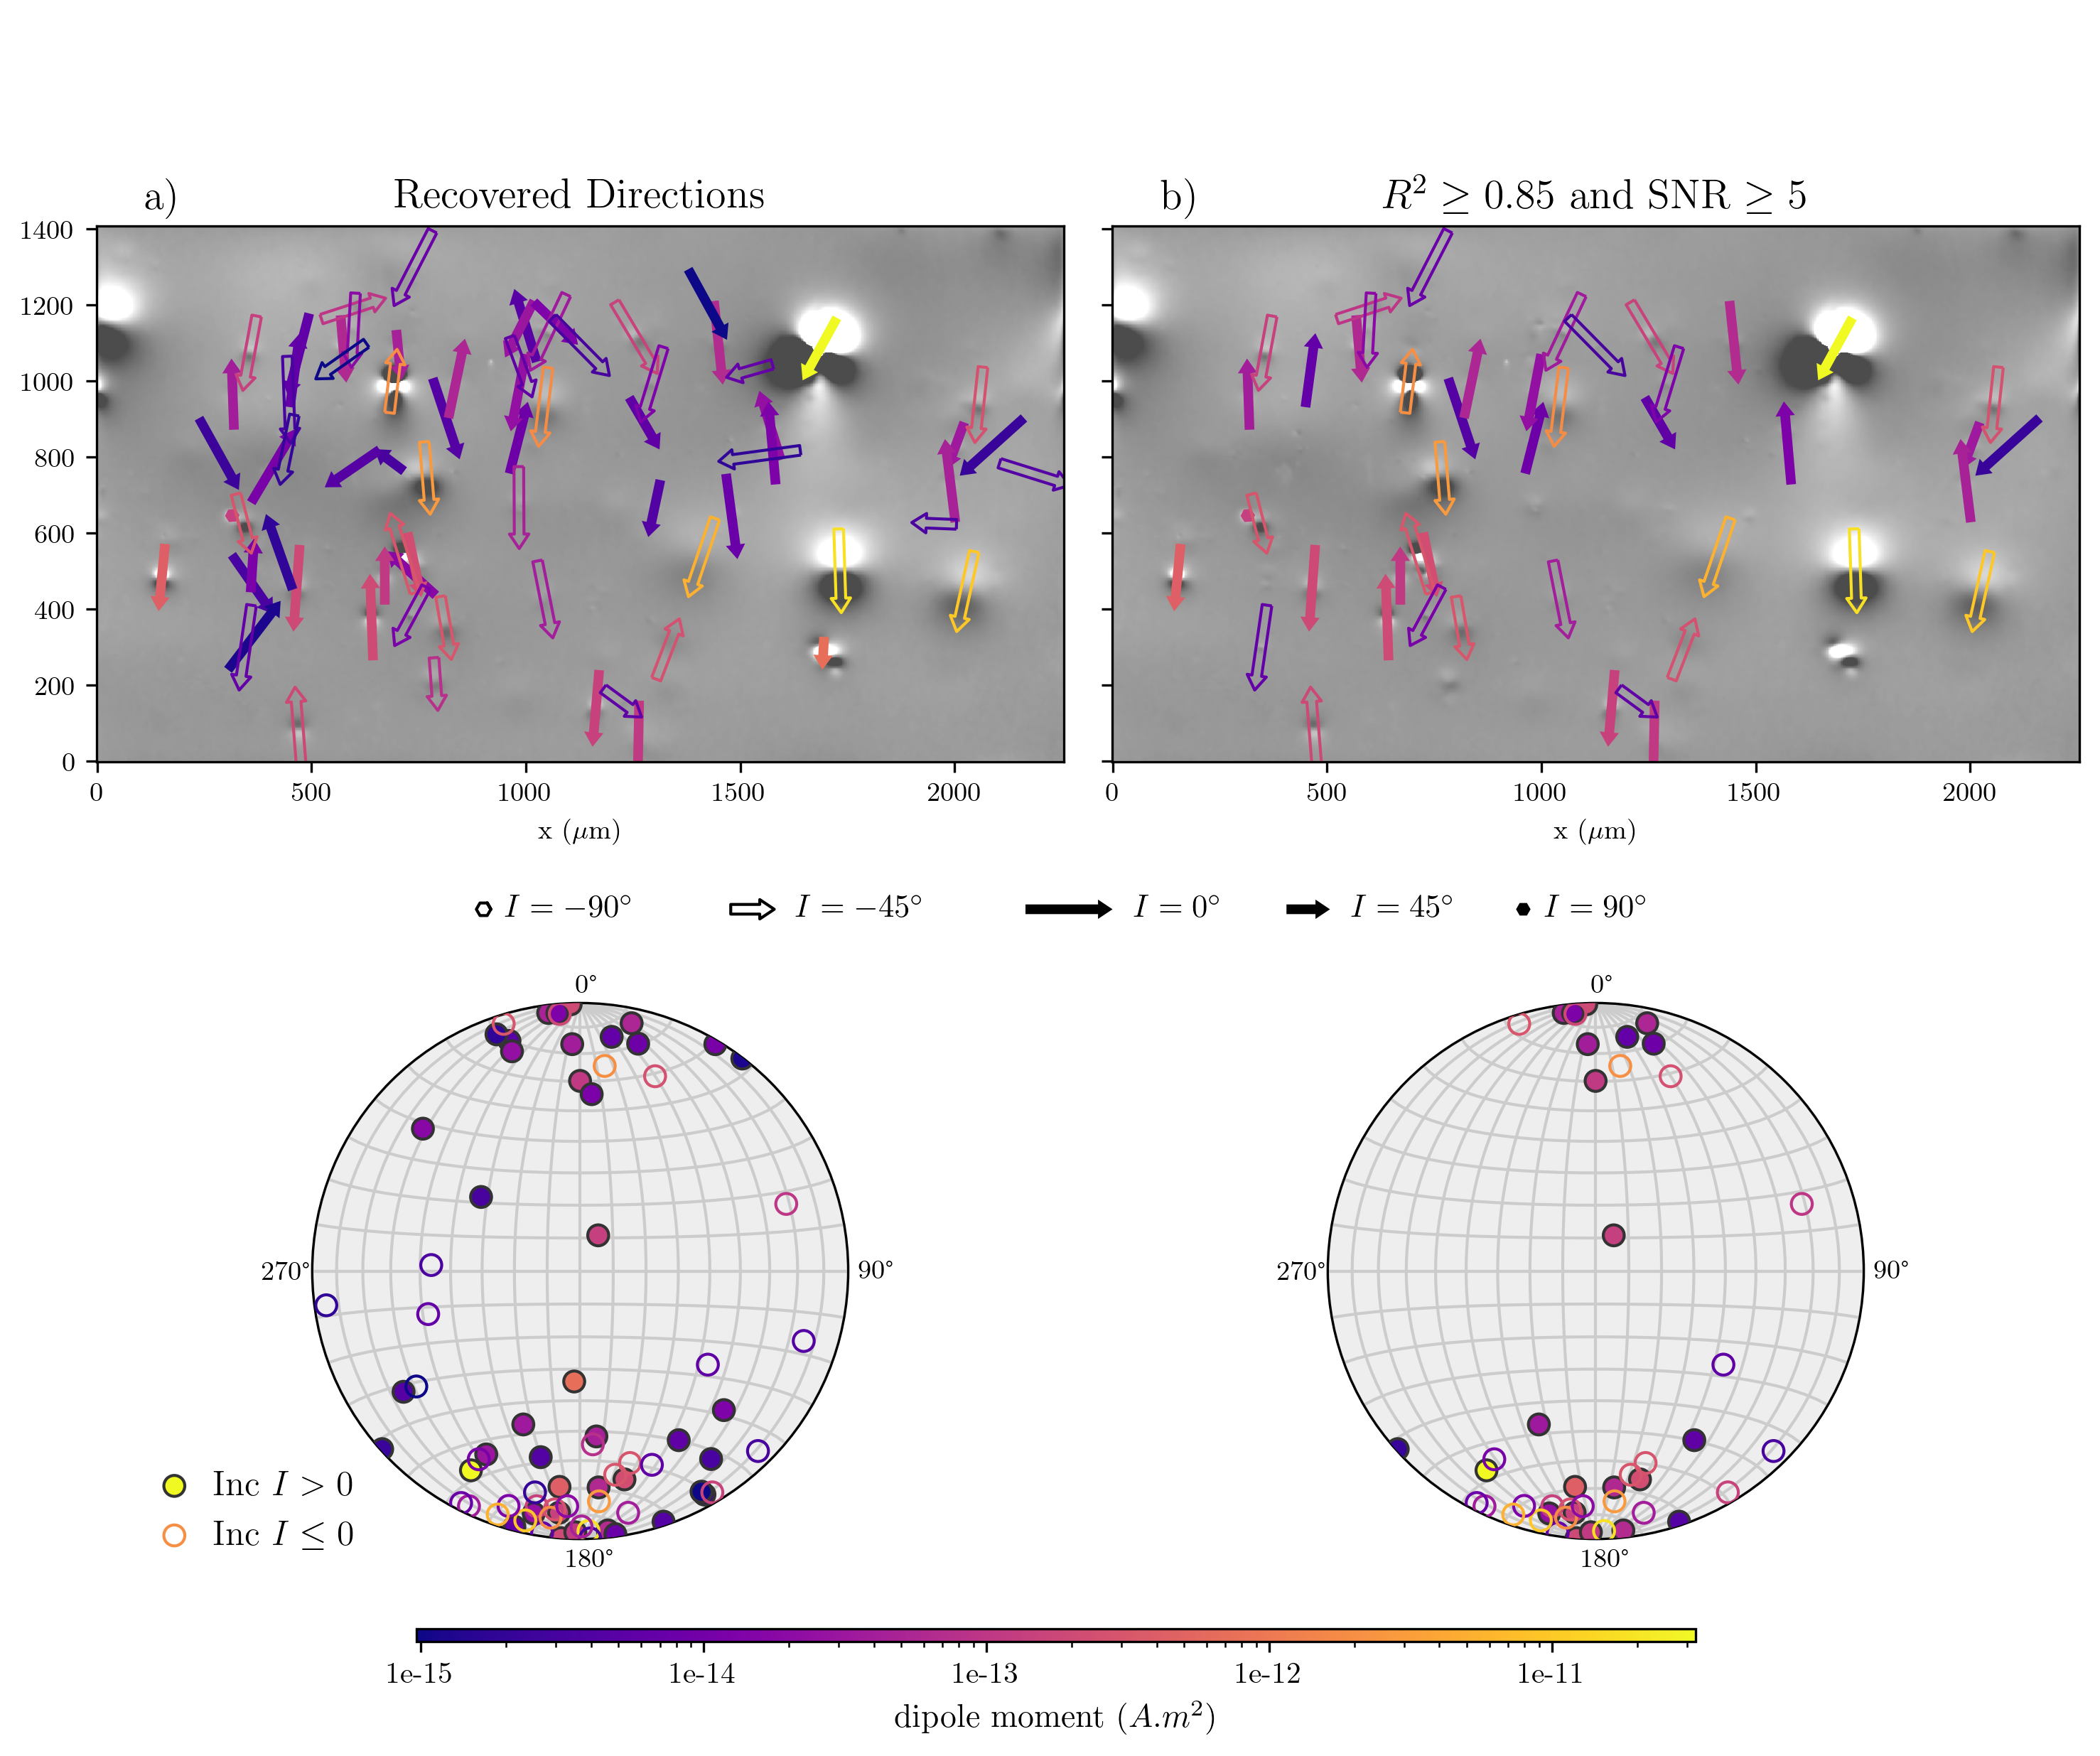
\includegraphics[width=1\linewidth]{figures/real-data-stereograms.png}
\caption{
Comparison of the estimated dipole magnetic moments and directions for the real data sample.
a) All estimated directions without filtering ($M=75$). b) Estimated directions filtered ($M=46$) by the coefficient of determination ($\geq 0.85$) and SNR ($\geq 5$), which shows two clusters of direction located on each pole of the stereogram.
}
\label{real-data-stereograms}
\end{figure}
